\documentclass{beamer}
% \documentclass[handout]{beamer}

\usepackage{amsmath,amsfonts,amsthm,amssymb,euscript,mathrsfs,url,stmaryrd,bbm}
\usepackage{subfigure}
\usepackage{tikz}

\usepackage{color}
\usepackage{import}

% \usepackage[absolute,overlay]{textpos}

\usepackage[utf8]{inputenc}

% should get rid of superfluous equation labels
% or all labels, if we never reference
\usepackage{mathtools}
\mathtoolsset{showonlyrefs}

\usepackage{multicol}
\usepackage{multirow}
\usepackage{colortbl}
\usepackage{booktabs}

% \usepackage[export]{adjustbox}% http://ctan.org/pkg/adjustbox


% theme
\usetheme{Singapore}
\useinnertheme{rounded}
\usecolortheme{rose}
% usetheme{Warsaw}

%farbversuche
%sieht sehr gut aus aber erstmal nicht
\definecolor{grey}{RGB}{0,0,0}
%aber wir machen erstmal was anderes
\definecolor{darkgreen}{RGB}{90,160,70}
\definecolor{darkred}{RGB}{160,70,70}
\definecolor{brickred}{RGB}{220,55,75}
% \definecolor{yellow}{RGB}{255,255,0}
\definecolor{turquoise}{RGB}{0,255,255}
% \definecolor{grey}{RGB}{0,255,255}
\definecolor{maroon}{RGB}{128,0,0}

%farbe als structure setzen
\setbeamercolor{structure}{fg=maroon!40!black}
% \setbeamercolor{structure}{fg=white!72!black}
%\setbeamercolor{structure}{fg=white!50!green!60!black}

%versuch die textfarbe zu setzen
% \setbeamercolor{normal text}{fg=blue!30!black}
%\setbeamercolor{normal text}{fg=blue}

% cover up
\setbeamercovered{transparent}

% make it work on matthias' laptop
% \setbeamertemplate{blocks}[default]


% macros
\renewcommand{\P}{\mathbb{P}}
\newcommand{\E}{\mathbb{E}}
\newcommand{\V}{\mathbb{V}}
% \newcommand{\N}{\ensuremath{\mathbb{N}}}
\newcommand{\R}{\ensuremath{\mathbb{R}}}
\newcommand{\1}{\ensuremath{\mathbf{1}}}
% \input{macros.tex}


% \newlength{\nodedist}


\setbeamercolor*{title}{use=structure,fg=white,bg=structure.fg,}
\setbeamertemplate{title page}[default][colsep=-4bp,rounded=true,shadow=true]

%we need this because sometimes we flip it
\def\defaultbeameritem{ball}
\setbeamertemplate{itemize items}[\defaultbeameritem]


% fancy footline
\setbeamertemplate{footline}
{

\begin{tikzpicture}(0,0)
\draw[draw=none,top color=white,bottom color=grey!20!white] (0,0) rectangle (\paperwidth,0.25);
% \node at (\paperwidth-12,0.2) {\insertframenumber /\inserttotalframenumber};
\node at (\paperwidth-12,0.2) {\insertpagenumber /\insertpresentationendpage};
\end{tikzpicture}}

%suppress navigation symbols
\setbeamertemplate{navigation symbols}{}
% % no footline
% \setbeamertemplate{footline}{}
% \setbeamertemplate{footline}[frame number]

% we want numbered figures
\setbeamertemplate{caption}[numbered]

% relevant stuff
\title{EMBO PopGen}
\subtitle{Coalescent theory}
\author{Matthias Steinrücken\\[2ex]{\scriptsize adapted from Matteo Fumagalli (EMBO, 2024)}}
% \institute{Department of Ecology and Evolution, University of Chicago\\ Department of Human Genetics, University of Chicago\\ NITMB} 
\institute{Department of Ecology and Evolution, University of Chicago\\ Department of Human Genetics, University of Chicago} 
\date{Day 2b, June 24, 2025}

\def\newblock{\hskip .11em plus .33em minus .07em}
\renewcommand{\raggedright}{\leftskip=0pt \rightskip=0pt plus 0cm} 
\renewcommand{\insertnavigation}[1]{\insertsectionnavigationhorizontal{#1}{}{}}



\begin{document}
%%%%%%%%%%%%%%%%%%%%%%%%%%%%%%%%%%%%%%%%%%%%%%%%%%%%%%%%%%%%%%%%%%%%%%%%%%%%%%%%%%%%%%
%
%
%
%%%%%%%%%%%%%%%%%%%%%%%%%%%%%%%%%%%%%%%%%%%%%%%%%%%%%%%%%%%%%%%%%%%%%%%%%%%%%%%%%%%%%%
\logo{\begin{minipage}[!b]{2cm}
\includegraphics[width=1.5cm]{graphics_day2b_popgen/university.seal.rgb.maroon.png}\\\phantom{a}\\\phantom{b}\end{minipage}}
%%%%%%%%%%%%%%%%%%%%%%%%%%%%%%%%%%%%%%%%%%%%%%%%%%%%%%%%%%%%%%%%%%%%%%%%%%%%%%%%%%%%%%
%
%
%
%%%%%%%%%%%%%%%%%%%%%%%%%%%%%%%%%%%%%%%%%%%%%%%%%%%%%%%%%%%%%%%%%%%%%%%%%%%%%%%%%%%%%%
\begin{frame}
	\titlepage 
	% \addtocounter{framenumber}{-1}
\end{frame}
\logo{}
%%%%%%%%%%%%%%%%%%%%%%%%%%%%%%%%%%%%%%%%%%%%%%%%%%%%%%%%%%%%%%%%%%%%%%%%%%%%%%%%%%%%%%
%
%
%
%%%%%%%%%%%%%%%%%%%%%%%%%%%%%%%%%%%%%%%%%%%%%%%%%%%%%%%%%%%%%%%%%%%%%%%%%%%%%%%%%%%%%%
\begin{frame}\frametitle{Intended Learning Outcomes}
	\textbf{Coalescent theory}\\[2ex]
	In this session you will learn:
	\begin{itemize}
		\item Describe principles and assumptions of coalescent theory.
		\item Discuss the infinite sites model.
		\item Provide estimators of $\theta$ and effective population size.
		\item Measure genetic variability with summary statistics and the site frequency spectrum.
	\end{itemize}
\end{frame}
%%%%%%%%%%%%%%%%%%%%%%%%%%%%%%%%%%%%%%%%%%%%%%%%%%%%%%%%%%%%%%%%%%%%%%%%%%%%%%%%%%%%%%
%
%
%
% %%%%%%%%%%%%%%%%%%%%%%%%%%%%%%%%%%%%%%%%%%%%%%%%%%%%%%%%%%%%%%%%%%%%%%%%%%%%%%%%%%%%%%
% \begin{frame}\frametitle{Motivation}
% 	\begin{center}
% 		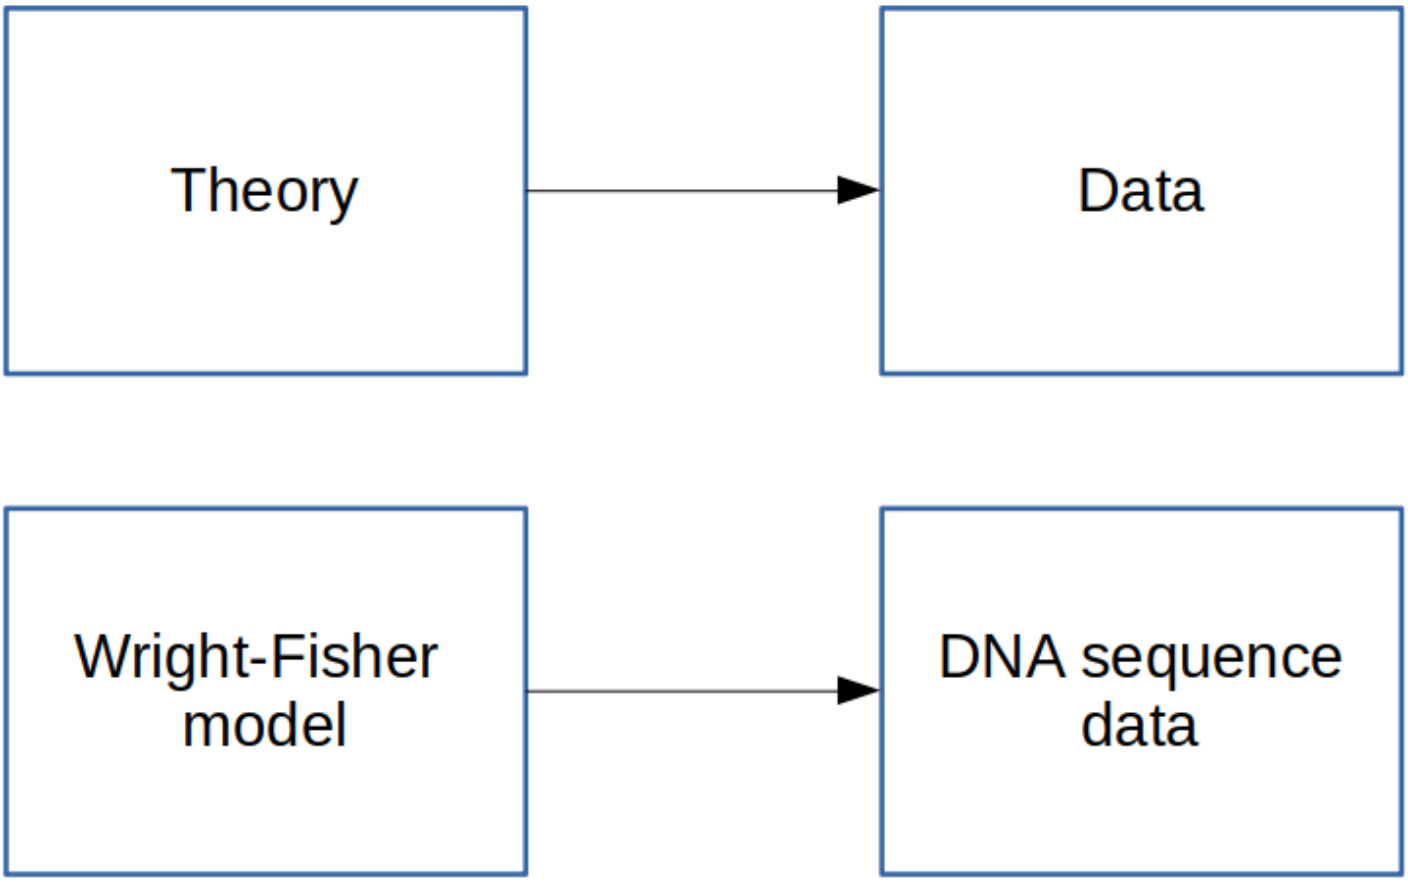
\includegraphics[width=.6\textwidth]{graphics_day2b_popgen/motivation.png}
% 	\end{center}
% \end{frame}
% %%%%%%%%%%%%%%%%%%%%%%%%%%%%%%%%%%%%%%%%%%%%%%%%%%%%%%%%%%%%%%%%%%%%%%%%%%%%%%%%%%%%%%
%
%
%
%%%%%%%%%%%%%%%%%%%%%%%%%%%%%%%%%%%%%%%%%%%%%%%%%%%%%%%%%%%%%%%%%%%%%%%%%%%%%%%%%%%%%%
\begin{frame}\frametitle{Motivation}
	Example question: On the X chromosomes, two Europeans differ, on average, at 0.08\% of sites, while individuals from African populations differ at 0.12\% of sites.\\[2ex]
	What do these numbers tell us \emph{about} the two populations?
\visible<2>{\begin{block}{}
		We use \textbf{coalescent theory}, which is based on the Wright-Fisher model, to consider the genealogical history of a sample and make inferences about the past instead of modelling changes of allele frequencies forward in time.
	\end{block}}
\end{frame}
%%%%%%%%%%%%%%%%%%%%%%%%%%%%%%%%%%%%%%%%%%%%%%%%%%%%%%%%%%%%%%%%%%%%%%%%%%%%%%%%%%%%%%
%
%
%
%%%%%%%%%%%%%%%%%%%%%%%%%%%%%%%%%%%%%%%%%%%%%%%%%%%%%%%%%%%%%%%%%%%%%%%%%%%%%%%%%%%%%%
\begin{frame}\frametitle{Coalescence}
	\begin{figure}
	\begin{center}
		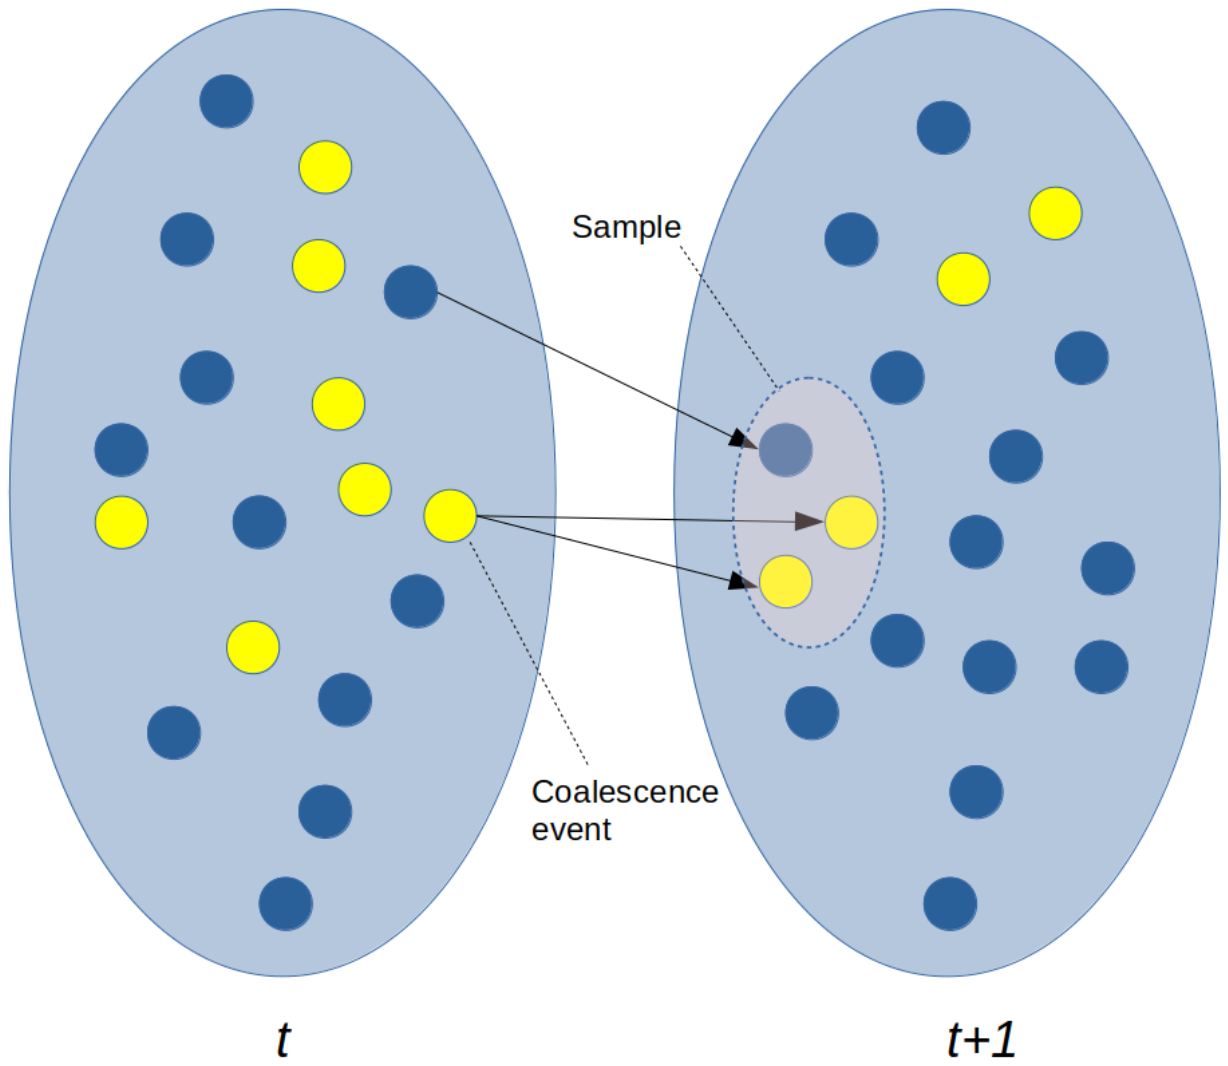
\includegraphics[width=.45\textwidth]{graphics_day2b_popgen/coalescence_event.png}
	\end{center}
	\caption{Tracking the ancestry of a sample between two generations.}
	\end{figure}
\end{frame}
%%%%%%%%%%%%%%%%%%%%%%%%%%%%%%%%%%%%%%%%%%%%%%%%%%%%%%%%%%%%%%%%%%%%%%%%%%%%%%%%%%%%%%
%
%
%
%%%%%%%%%%%%%%%%%%%%%%%%%%%%%%%%%%%%%%%%%%%%%%%%%%%%%%%%%%%%%%%%%%%%%%%%%%%%%%%%%%%%%%
\begin{frame}\frametitle{Coalescence}
	If two individual gene copies have the same parent in the previous generation, we say that the \textbf{ancestral lineages} representing these two individuals have \textbf{coalesced}.\\[2ex]
	They have a \textbf{common ancestor} and a \textbf{coalescent event} has occurred.
\end{frame}
%%%%%%%%%%%%%%%%%%%%%%%%%%%%%%%%%%%%%%%%%%%%%%%%%%%%%%%%%%%%%%%%%%%%%%%%%%%%%%%%%%%%%%
%
%
%
%%%%%%%%%%%%%%%%%%%%%%%%%%%%%%%%%%%%%%%%%%%%%%%%%%%%%%%%%%%%%%%%%%%%%%%%%%%%%%%%%%%%%%
\begin{frame}\frametitle{Coalescent tree}
	\begin{figure}
	\begin{center}
		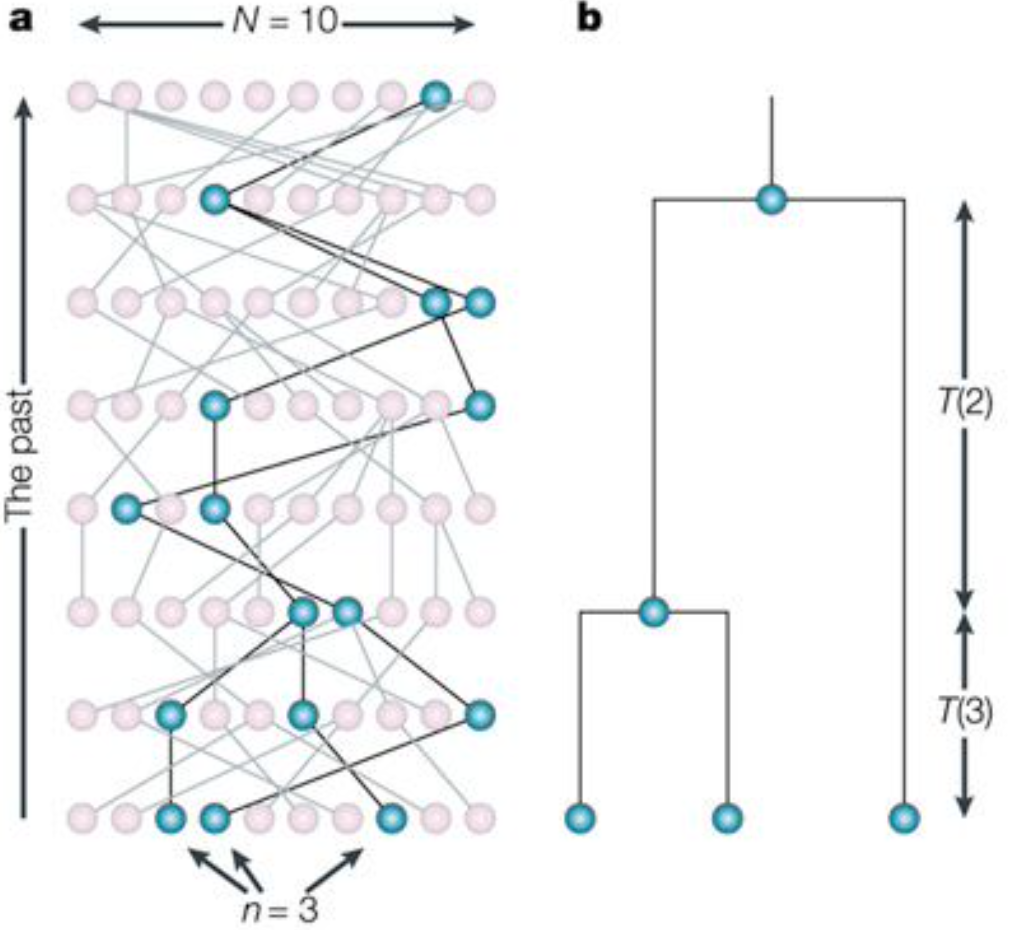
\includegraphics[width=.45\textwidth]{graphics_day2b_popgen/coalescent_tree.png}
	\end{center}
	\caption{Ancestry of three samples.}
	\end{figure}
\end{frame}
%%%%%%%%%%%%%%%%%%%%%%%%%%%%%%%%%%%%%%%%%%%%%%%%%%%%%%%%%%%%%%%%%%%%%%%%%%%%%%%%%%%%%%
%
%
%
%%%%%%%%%%%%%%%%%%%%%%%%%%%%%%%%%%%%%%%%%%%%%%%%%%%%%%%%%%%%%%%%%%%%%%%%%%%%%%%%%%%%%%
\begin{frame}\frametitle{Coalescent tree}
	The ancestry of an individual gene copy is represented by a lineage.\\[1.5ex]
	\begin{block}{}
		The time until two lineages find a \textbf{most recent common ancestor (MRCA)} is called \textbf{coalescence time}.
	\end{block}
	How can we find the coalescence time?
\end{frame}
%%%%%%%%%%%%%%%%%%%%%%%%%%%%%%%%%%%%%%%%%%%%%%%%%%%%%%%%%%%%%%%%%%%%%%%%%%%%%%%%%%%%%%
%
%
%
%%%%%%%%%%%%%%%%%%%%%%%%%%%%%%%%%%%%%%%%%%%%%%%%%%%%%%%%%%%%%%%%%%%%%%%%%%%%%%%%%%%%%%
\begin{frame}\frametitle{Coalescence in a sample of two gene copies}
	As there are $2N$ potential parents ``chosen'' with equal probability, the probability of two individuals having the same parent in the previous generation is:
\visible<2-4>{\begin{equation}
		1/(2N)
	\end{equation}%\\[2ex]
	The probability that two gene copies did NOT have the same parent in the previous generation is:
\visible<3-4>{\begin{equation}
		1-1/(2N)
	\end{equation}%\\[2ex]
	The probability that two gene copies did not have the same parent in the past r generations is:
\visible<4>{\begin{equation}
		[1 - 1/(2N)]^r
	\end{equation}}}}
\end{frame}
%%%%%%%%%%%%%%%%%%%%%%%%%%%%%%%%%%%%%%%%%%%%%%%%%%%%%%%%%%%%%%%%%%%%%%%%%%%%%%%%%%%%%%
%
%
%
%%%%%%%%%%%%%%%%%%%%%%%%%%%%%%%%%%%%%%%%%%%%%%%%%%%%%%%%%%%%%%%%%%%%%%%%%%%%%%%%%%%%%%
\begin{frame}\frametitle{Coalescence in a sample of two gene copies}
	The probability of not finding any common ancestor in generation $r-1$ but then finding the first common ancestor in generation r is:
\visible<2>{\begin{equation}
		\P(\ldots) = [1-1/(2N)]^{r-1}[1/(2N)]
	\end{equation}
	\begin{block}{}
		This equation gives us the probability distribution of the time to the MRCA in a sample of size $n = 2$. This is a \textbf{geometric} random variable: the probability distribution of the number of Bernoulli trials needed to get one success (w.p.\ $1/2N$).}
	\end{block}
\end{frame}
%%%%%%%%%%%%%%%%%%%%%%%%%%%%%%%%%%%%%%%%%%%%%%%%%%%%%%%%%%%%%%%%%%%%%%%%%%%%%%%%%%%%%%
%
%
%
%%%%%%%%%%%%%%%%%%%%%%%%%%%%%%%%%%%%%%%%%%%%%%%%%%%%%%%%%%%%%%%%%%%%%%%%%%%%%%%%%%%%%%
\begin{frame}\frametitle{Coalescence in a sample of two gene copies}
	\begin{figure}
	\begin{center}
		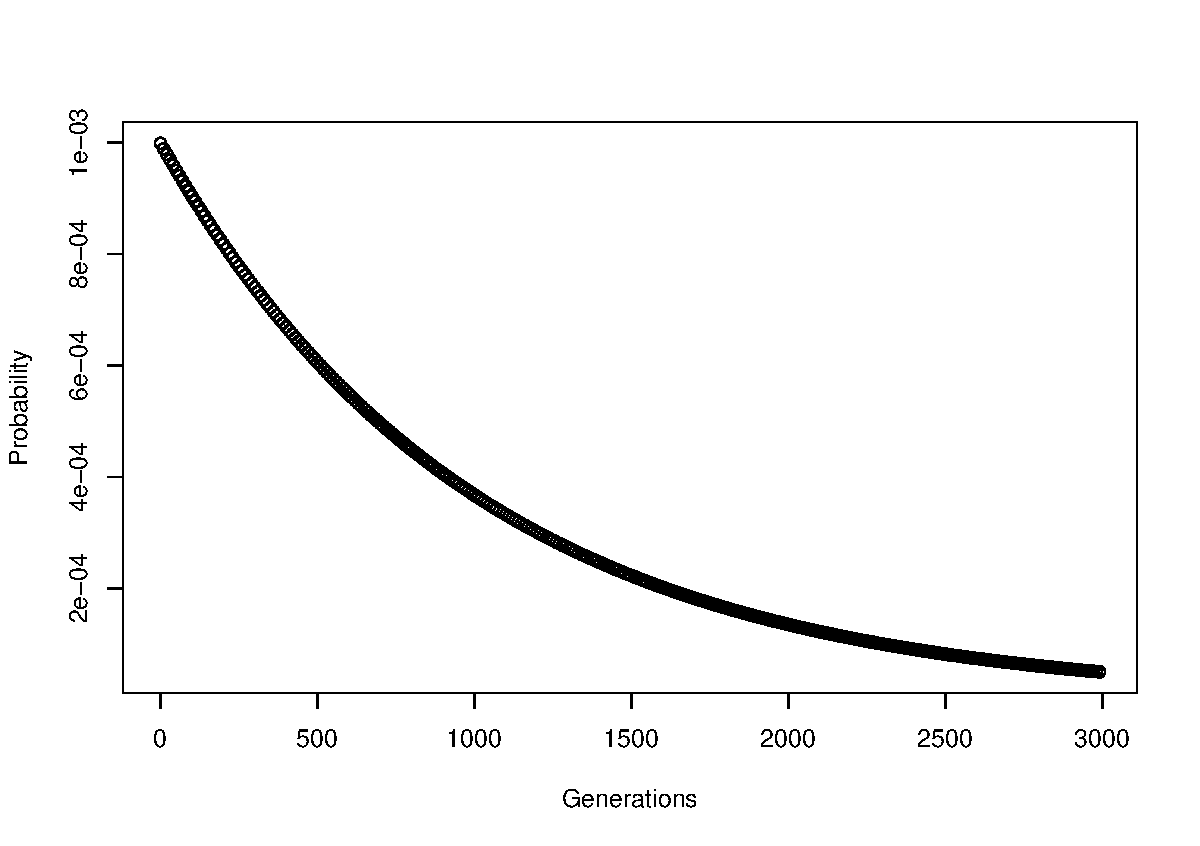
\includegraphics[width=.55\textwidth]{graphics_day2b_popgen/discrete_tmrca.pdf}
	\end{center}
	\caption{Distribution of TMRCA for $n=2$ in population of size $N=500$.}
	\end{figure}
\end{frame}
%%%%%%%%%%%%%%%%%%%%%%%%%%%%%%%%%%%%%%%%%%%%%%%%%%%%%%%%%%%%%%%%%%%%%%%%%%%%%%%%%%%%%%
%
%
%
%%%%%%%%%%%%%%%%%%%%%%%%%%%%%%%%%%%%%%%%%%%%%%%%%%%%%%%%%%%%%%%%%%%%%%%%%%%%%%%%%%%%%%
\begin{frame}\frametitle{Coalescence in large populations}
	\begin{itemize}
		\item If we consider the limit of an infinitely large population, calculations simplify but we can still consider the effect of genetic drift.
		\item It is convenient to measure time in $2N$ generations, by setting $r = 2Nt$ with $t$ measuring time in $2N$ generations.
	\end{itemize}
\visible<2>{\vspace{1ex}The probability that two gene copies do not find a common ancestor in $2Nt$ generations becomes
	\begin{equation}
		[1-1/(2N)]^{2Nt} \to e^{-t} \text{ as }N \to \infty
	\end{equation}}
\end{frame}
%%%%%%%%%%%%%%%%%%%%%%%%%%%%%%%%%%%%%%%%%%%%%%%%%%%%%%%%%%%%%%%%%%%%%%%%%%%%%%%%%%%%%%
%
%
%
%%%%%%%%%%%%%%%%%%%%%%%%%%%%%%%%%%%%%%%%%%%%%%%%%%%%%%%%%%%%%%%%%%%%%%%%%%%%%%%%%%%%%%
\begin{frame}\frametitle{Coalescence in large populations}
	As N becomes large, the distribution of the coalescence times follows an \textbf{exponential distribution} with mean 1.\\[2ex]
	As time is measured in $2N$ generations, the mean (expected) time to coalescence is actually $2N$ generations. In other words, there is a constant rate of coalescence of 1 per $2N$ generations.
\end{frame}
%%%%%%%%%%%%%%%%%%%%%%%%%%%%%%%%%%%%%%%%%%%%%%%%%%%%%%%%%%%%%%%%%%%%%%%%%%%%%%%%%%%%%%
%
%
%
%%%%%%%%%%%%%%%%%%%%%%%%%%%%%%%%%%%%%%%%%%%%%%%%%%%%%%%%%%%%%%%%%%%%%%%%%%%%%%%%%%%%%%
\begin{frame}\frametitle{Coalescence in large populations}
	\begin{figure}
	\begin{center}
		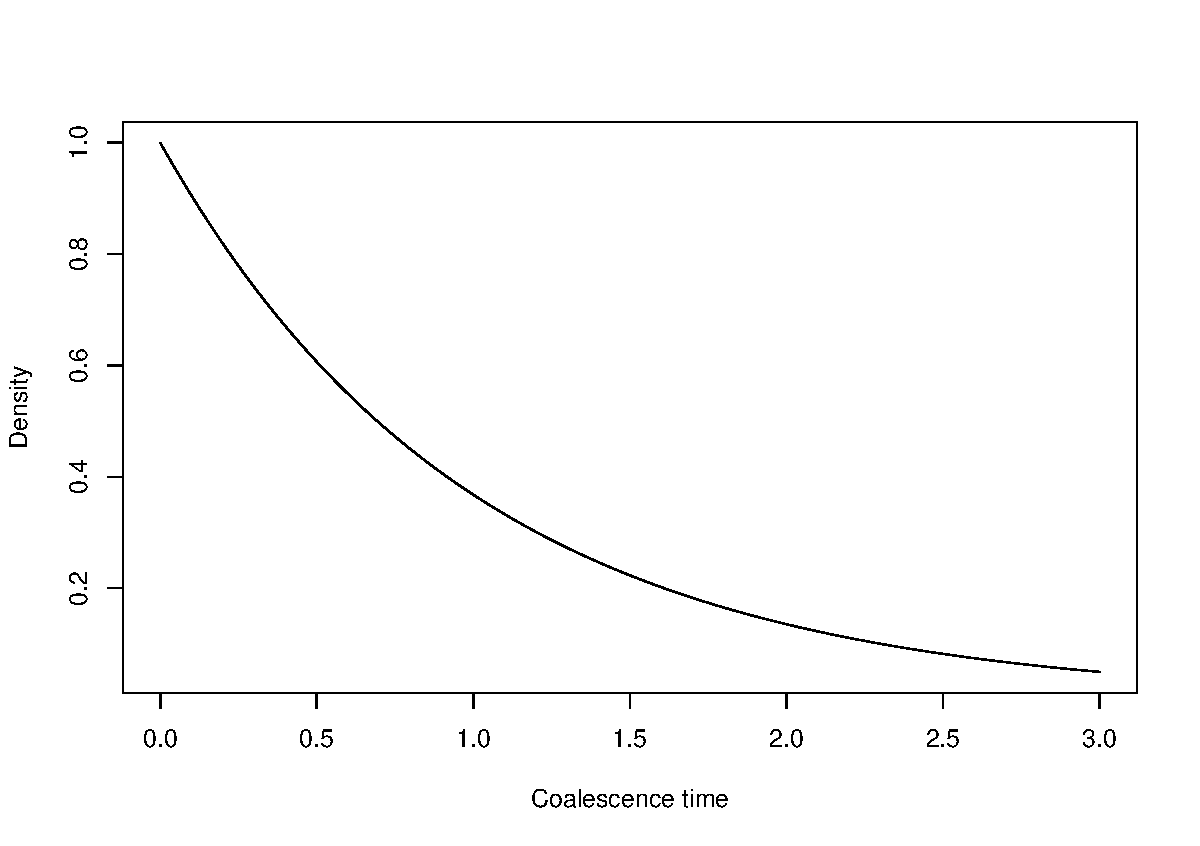
\includegraphics[width=.55\textwidth]{graphics_day2b_popgen/continuous_tmrca.pdf}
	\end{center}
	\caption{Exponential distribution of TMRCA for $n=2$. Time $t=1$ corresponds to $2N$ generations.}
	\end{figure}
\end{frame}
%%%%%%%%%%%%%%%%%%%%%%%%%%%%%%%%%%%%%%%%%%%%%%%%%%%%%%%%%%%%%%%%%%%%%%%%%%%%%%%%%%%%%%
%
%
%
%%%%%%%%%%%%%%%%%%%%%%%%%%%%%%%%%%%%%%%%%%%%%%%%%%%%%%%%%%%%%%%%%%%%%%%%%%%%%%%%%%%%%%
\begin{frame}\frametitle{Coalescence in large populations}
	\begin{itemize}
		\item The random process of following the lineages backward in time until a most recent common ancestor has been found is called the \textbf{coalescence process}.
		\item If the coalescence rate is 1 per $2N$ generations, it is intuitive to understand that the expected coalescence time (the time until the coalescent event occurs) is $2N$ generations (although there is considerable variability in the coalescence times).
	\end{itemize}
\end{frame}
%%%%%%%%%%%%%%%%%%%%%%%%%%%%%%%%%%%%%%%%%%%%%%%%%%%%%%%%%%%%%%%%%%%%%%%%%%%%%%%%%%%%%%
%
%
%
%%%%%%%%%%%%%%%%%%%%%%%%%%%%%%%%%%%%%%%%%%%%%%%%%%%%%%%%%%%%%%%%%%%%%%%%%%%%%%%%%%%%%%
\begin{frame}\frametitle{Coalescence in large populations}
	\begin{itemize}
		\item The coalescence process in a large randomly mating diploid population with two sexes is the same as that in the simple haploid model.
		\item Once we have a convenient description of the geneaology, then it is easy to derive various properties of our sample.
	\end{itemize}
\end{frame}
%%%%%%%%%%%%%%%%%%%%%%%%%%%%%%%%%%%%%%%%%%%%%%%%%%%%%%%%%%%%%%%%%%%%%%%%%%%%%%%%%%%%%%
%
%
%
%%%%%%%%%%%%%%%%%%%%%%%%%%%%%%%%%%%%%%%%%%%%%%%%%%%%%%%%%%%%%%%%%%%%%%%%%%%%%%%%%%%%%%
\begin{frame}\frametitle{Coalescence in large populations}
	\begin{columns}
	\begin{column}{.33\textwidth}
		\begin{center}
			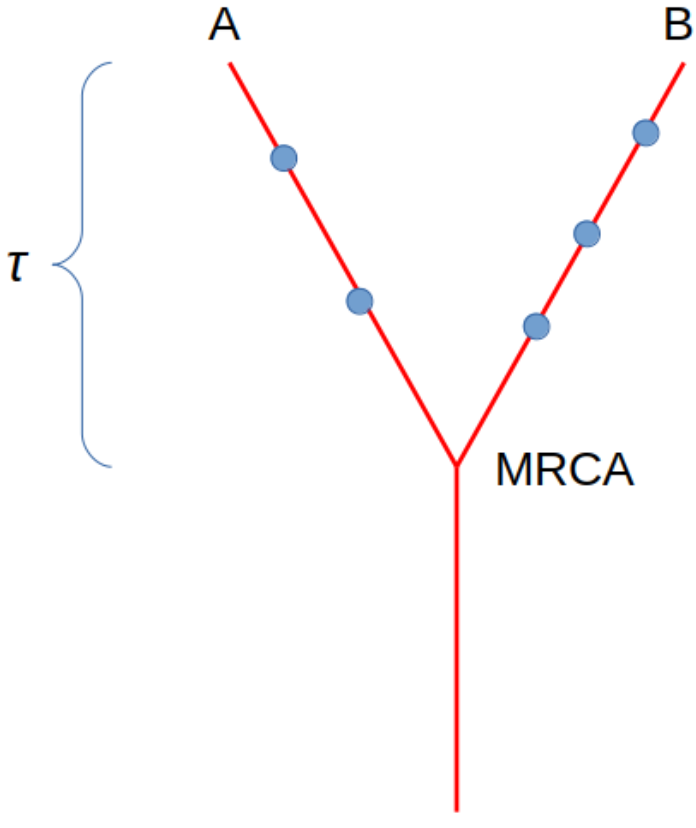
\includegraphics[width=\textwidth]{graphics_day2b_popgen/coalescent_fork.png}
		\end{center}
	\end{column}
	\begin{column}{.66\textwidth}
\only<1>{We expect $\mu r$ mutations in $r$ generations. If we measure time by $2N$ generations, that is $t = r/(2N)$, we expect $2N\mu t$ mutations on a lineage of length $t$.\\[1.5ex]
		Since $\E[t] = 1$ and there are two lineages, the expected number of mutations separating two gene copies is
		\begin{block}{}
		\begin{equation}
			\theta = 4N\mu
		\end{equation}
		\end{block}
		which is a simple relationship between the amount of genetic variability, mutation rate, and population size.}
\only<2>{\hspace{-.5em}The expected number of mutations occurring on a lineage during any time interval of length $\tau$ is $2N\mu \tau = \tau\theta/2$.\\[1.5ex]
As such, we can think of the data generated by a coalescence process producing a coalescent tree and a subsequent process in which mutations are distributed across the lineages of the tree at rate $\theta/2$.}
	\end{column}
	\end{columns}
\end{frame}
%%%%%%%%%%%%%%%%%%%%%%%%%%%%%%%%%%%%%%%%%%%%%%%%%%%%%%%%%%%%%%%%%%%%%%%%%%%%%%%%%%%%%%
%
%
%
%%%%%%%%%%%%%%%%%%%%%%%%%%%%%%%%%%%%%%%%%%%%%%%%%%%%%%%%%%%%%%%%%%%%%%%%%%%%%%%%%%%%%%
\begin{frame}\frametitle{Infinite Sites Model}
	\begin{block}{}
		Each new mutation creates a new variable site, i.e.\ each new mutation hits a new site in the sequence, such that no site experiences more than one mutation.
	\end{block}
	\begin{figure}
	\begin{center}
		
\includegraphics[width=.9\textwidth]{graphics_day2b_popgen/infinte_sites_model.png}
	\end{center}
	\caption{The sequence is infinitely long so that the chance of two mutations hit the same site is essentially zero.}
	\end{figure}
\end{frame}
%%%%%%%%%%%%%%%%%%%%%%%%%%%%%%%%%%%%%%%%%%%%%%%%%%%%%%%%%%%%%%%%%%%%%%%%%%%%%%%%%%%%%%
%
%
%
%%%%%%%%%%%%%%%%%%%%%%%%%%%%%%%%%%%%%%%%%%%%%%%%%%%%%%%%%%%%%%%%%%%%%%%%%%%%%%%%%%%%%%
\begin{frame}\frametitle{Infinite Sites Model}
	The sites at which some of the individuals differ are called \textbf{segregating sites} or \textbf{single nucleotide polymorphisms} (SNPs).
	\begin{center}
		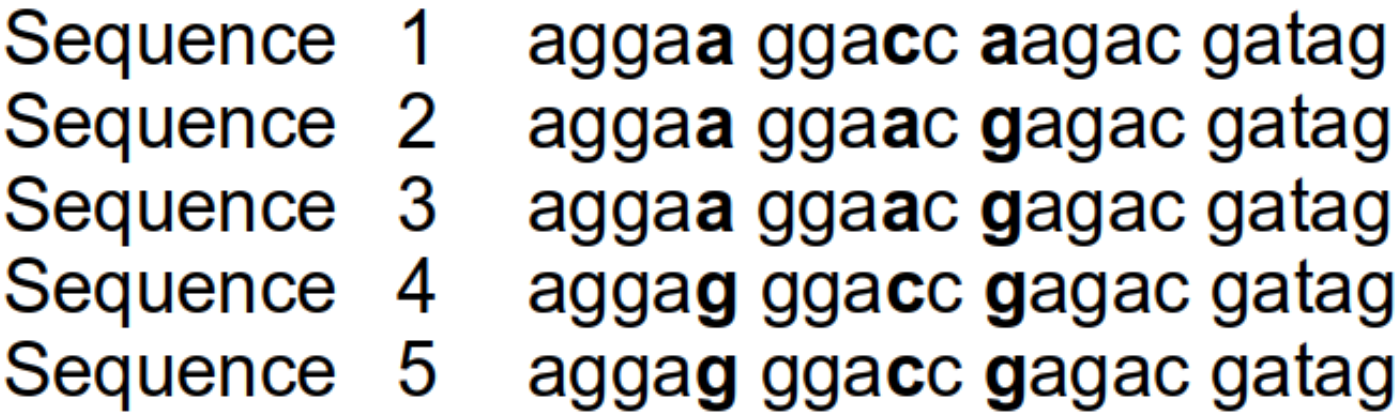
\includegraphics[width=.7\textwidth]{graphics_day2b_popgen/ims_sequences.png}
	\end{center}
	Under the infinite sites model, we can deduce which mutations occurred in the ancestry of a sample of sequences.
\end{frame}
%%%%%%%%%%%%%%%%%%%%%%%%%%%%%%%%%%%%%%%%%%%%%%%%%%%%%%%%%%%%%%%%%%%%%%%%%%%%%%%%%%%%%%
%
%
%
%%%%%%%%%%%%%%%%%%%%%%%%%%%%%%%%%%%%%%%%%%%%%%%%%%%%%%%%%%%%%%%%%%%%%%%%%%%%%%%%%%%%%%
\begin{frame}\frametitle{Infinite Sites Model}
	The model does not distinguish between different nucleotides and does not care about invariable sites.
	\begin{figure}
	\begin{center}
		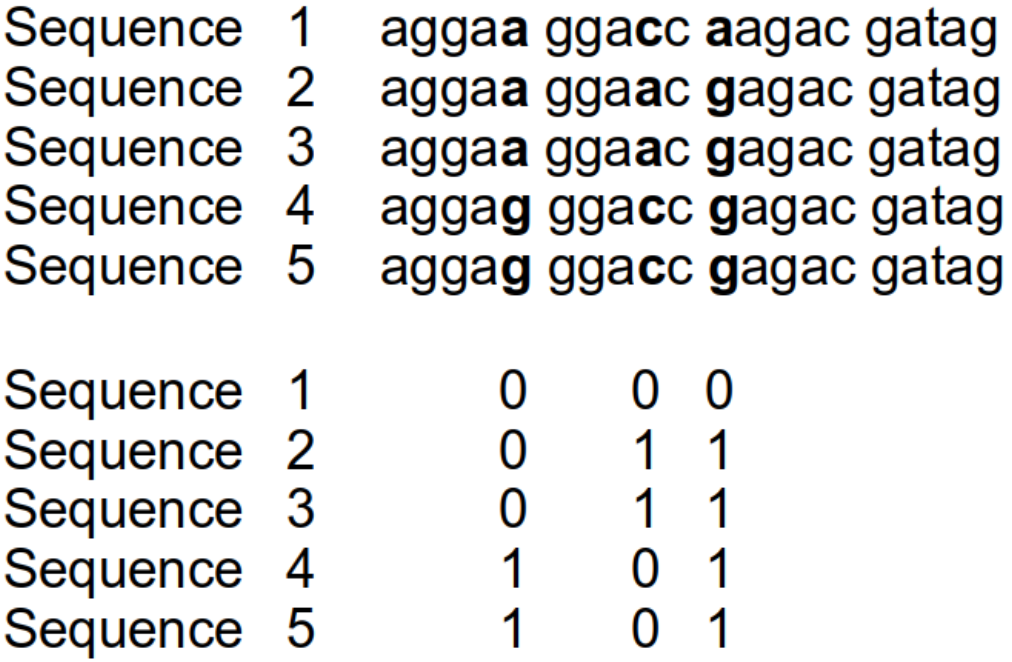
\includegraphics[width=.6\textwidth]{graphics_day2b_popgen/ims_sequences_matrix.png}
	\end{center}
	\caption{Data as a binary matrix of the variable sites.}
	\end{figure}
\end{frame}
%%%%%%%%%%%%%%%%%%%%%%%%%%%%%%%%%%%%%%%%%%%%%%%%%%%%%%%%%%%%%%%%%%%%%%%%%%%%%%%%%%%%%%
%
%
%
%%%%%%%%%%%%%%%%%%%%%%%%%%%%%%%%%%%%%%%%%%%%%%%%%%%%%%%%%%%%%%%%%%%%%%%%%%%%%%%%%%%%%%
\begin{frame}\frametitle{Infinite Sites Model}
	\begin{itemize}
		\item Labelling with zeros and ones is arbitrary.
		\item Good approximation if the rate of mutation is low.
		\item DNA sequences with different mutations are different \textbf{haplotypes}.
	\end{itemize}
	\begin{figure}
	\begin{center}
		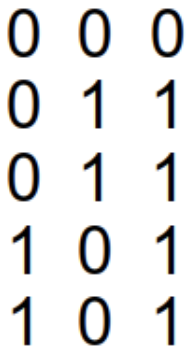
\includegraphics[width=.1\textwidth]{graphics_day2b_popgen/small_ims_matrix.png}
	\end{center}
	\caption{How many DNA sequences? How many haplotypes?}
	\end{figure}
\end{frame}
%%%%%%%%%%%%%%%%%%%%%%%%%%%%%%%%%%%%%%%%%%%%%%%%%%%%%%%%%%%%%%%%%%%%%%%%%%%%%%%%%%%%%%
%
%
%
%%%%%%%%%%%%%%%%%%%%%%%%%%%%%%%%%%%%%%%%%%%%%%%%%%%%%%%%%%%%%%%%%%%%%%%%%%%%%%%%%%%%%%
\begin{frame}\frametitle{Tajima’s estimator}
	We want an estimate of $\theta = 4N\mu$ under the infinite sites model from the expected number of mutations separating two individuals based on the DNA sequences obtained from data.\\[2ex]
\visible<2>{
	Data can be summarised as the \textbf{average number of pairwise differences}, or $\pi$.
	\begin{equation}
		\pi = \frac{\sum_{i<j}d_{i,j}}{n(n-1)/2}
	\end{equation}
	with $n$ sequences, $d_{i,j}$ number of differences between sequence $i$ and $j$.
}
\end{frame}
%%%%%%%%%%%%%%%%%%%%%%%%%%%%%%%%%%%%%%%%%%%%%%%%%%%%%%%%%%%%%%%%%%%%%%%%%%%%%%%%%%%%%%
%
%
%
%%%%%%%%%%%%%%%%%%%%%%%%%%%%%%%%%%%%%%%%%%%%%%%%%%%%%%%%%%%%%%%%%%%%%%%%%%%%%%%%%%%%%%
\begin{frame}\frametitle{Tajima’s estimator}
	\begin{figure}
	\begin{center}
		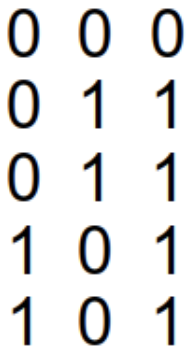
\includegraphics[width=.1\textwidth]{graphics_day2b_popgen/small_ims_matrix.png}
	\end{center}
	\caption{What is the value of $\pi$?}
	\end{figure}
\visible<2>{$\pi = (2 + 2 + 2 + 2 + 0 + 2 + 2 + 2 + 2 + 0)/(5 \times 4/2) = 1.6$}
\end{frame}
%%%%%%%%%%%%%%%%%%%%%%%%%%%%%%%%%%%%%%%%%%%%%%%%%%%%%%%%%%%%%%%%%%%%%%%%%%%%%%%%%%%%%%
%
%
%
%%%%%%%%%%%%%%%%%%%%%%%%%%%%%%%%%%%%%%%%%%%%%%%%%%%%%%%%%%%%%%%%%%%%%%%%%%%%%%%%%%%%%%
\begin{frame}\frametitle{Coalescence in large populations}
	\begin{columns}
	\begin{column}{.33\textwidth}
		\begin{center}
			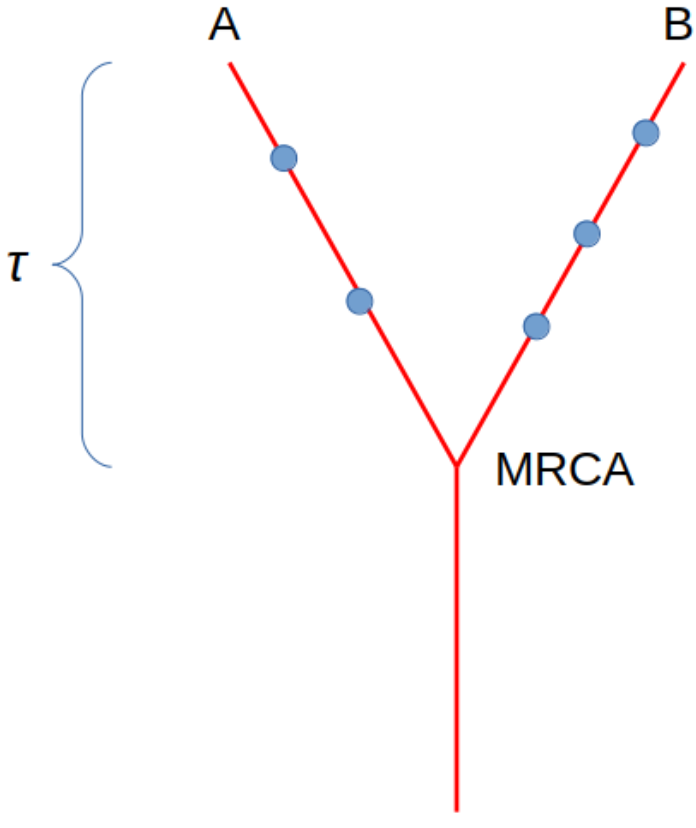
\includegraphics[width=\textwidth]{graphics_day2b_popgen/coalescent_fork.png}
		\end{center}
	\end{column}
	\begin{column}{.66\textwidth}
		The expected number of nucleotide differences between two sequences is the expected number of mutations, $\theta = 4N\mu$.
		\begin{equation}
			\E[d_{i,j}] = \theta
		\end{equation}
		\begin{equation}
			\E[\pi] = \theta
		\end{equation}
		$\hat\theta = \pi$ is called Tajima’s estimator of $\theta$.
	\end{column}
	\end{columns}
\end{frame}
%%%%%%%%%%%%%%%%%%%%%%%%%%%%%%%%%%%%%%%%%%%%%%%%%%%%%%%%%%%%%%%%%%%%%%%%%%%%%%%%%%%%%%
%
%
%
%%%%%%%%%%%%%%%%%%%%%%%%%%%%%%%%%%%%%%%%%%%%%%%%%%%%%%%%%%%%%%%%%%%%%%%%%%%%%%%%%%%%%%
\begin{frame}\frametitle{Watterson’s estimator}
	\begin{equation}
		\hat{\theta}_W = \frac{S}{\sum_{k=1}^{n-1}\tfrac{1}{k}}
	\end{equation}
	with $S$ segregating sites in $n$ samples.
	\begin{equation}
		\E [\hat{\theta}_W] = \theta
	\end{equation}
\end{frame}
%%%%%%%%%%%%%%%%%%%%%%%%%%%%%%%%%%%%%%%%%%%%%%%%%%%%%%%%%%%%%%%%%%%%%%%%%%%%%%%%%%%%%%
%
%
%
%%%%%%%%%%%%%%%%%%%%%%%%%%%%%%%%%%%%%%%%%%%%%%%%%%%%%%%%%%%%%%%%%%%%%%%%%%%%%%%%%%%%%%
\begin{frame}\frametitle{Watterson’s estimator}
	\begin{figure}
	\begin{center}
		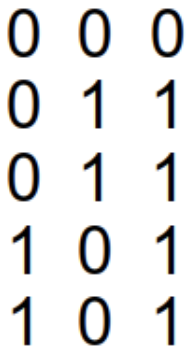
\includegraphics[width=.1\textwidth]{graphics_day2b_popgen/small_ims_matrix.png}
	\end{center}
	\caption{What is the value of $\hat\theta_W$?}
	\end{figure}
\visible<2>{$\hat\theta_W = 3/(1+1/2+1/3+1/4) = 1.4$\\
	but before we obtained $\hat\theta_T = 1.6$.\\
	Why?}
\end{frame}
%%%%%%%%%%%%%%%%%%%%%%%%%%%%%%%%%%%%%%%%%%%%%%%%%%%%%%%%%%%%%%%%%%%%%%%%%%%%%%%%%%%%%%
%
%
%
%%%%%%%%%%%%%%%%%%%%%%%%%%%%%%%%%%%%%%%%%%%%%%%%%%%%%%%%%%%%%%%%%%%%%%%%%%%%%%%%%%%%%%
\begin{frame}\frametitle{Effective population size ($N_e$)}
	\begin{block}{}
		The number of individuals in the Wright-Fisher model that would produce the same amount of genetic drift as in the real population.
	\end{block}
	The amount of genetic drift can be measured as
	\begin{itemize}
		\item Expected heterozygosity,
		\item Expected number of pairwise differences ($\approx \theta$).
		\item Rate of coalescence.
		\item ...
	\end{itemize}
\end{frame}
%%%%%%%%%%%%%%%%%%%%%%%%%%%%%%%%%%%%%%%%%%%%%%%%%%%%%%%%%%%%%%%%%%%%%%%%%%%%%%%%%%%%%%
%
%
%
%%%%%%%%%%%%%%%%%%%%%%%%%%%%%%%%%%%%%%%%%%%%%%%%%%%%%%%%%%%%%%%%%%%%%%%%%%%%%%%%%%%%%%
\begin{frame}\frametitle{Effective population size ($N_e$)}
	E.g.\ \emph{``A population with an effective size of 200 with respect to heterozygosity harbours the same amount of heterozygosity as a Wright-Fisher population of 200 individuals.''}\\[2ex]
	The true number of individuals in the population can be very different from its effective population size! (Often a lot larger.)
\end{frame}
%%%%%%%%%%%%%%%%%%%%%%%%%%%%%%%%%%%%%%%%%%%%%%%%%%%%%%%%%%%%%%%%%%%%%%%%%%%%%%%%%%%%%%
%
%
%
%%%%%%%%%%%%%%%%%%%%%%%%%%%%%%%%%%%%%%%%%%%%%%%%%%%%%%%%%%%%%%%%%%%%%%%%%%%%%%%%%%%%%%
\begin{frame}\frametitle{Effective population size}
	\begin{figure}
	\begin{center}
		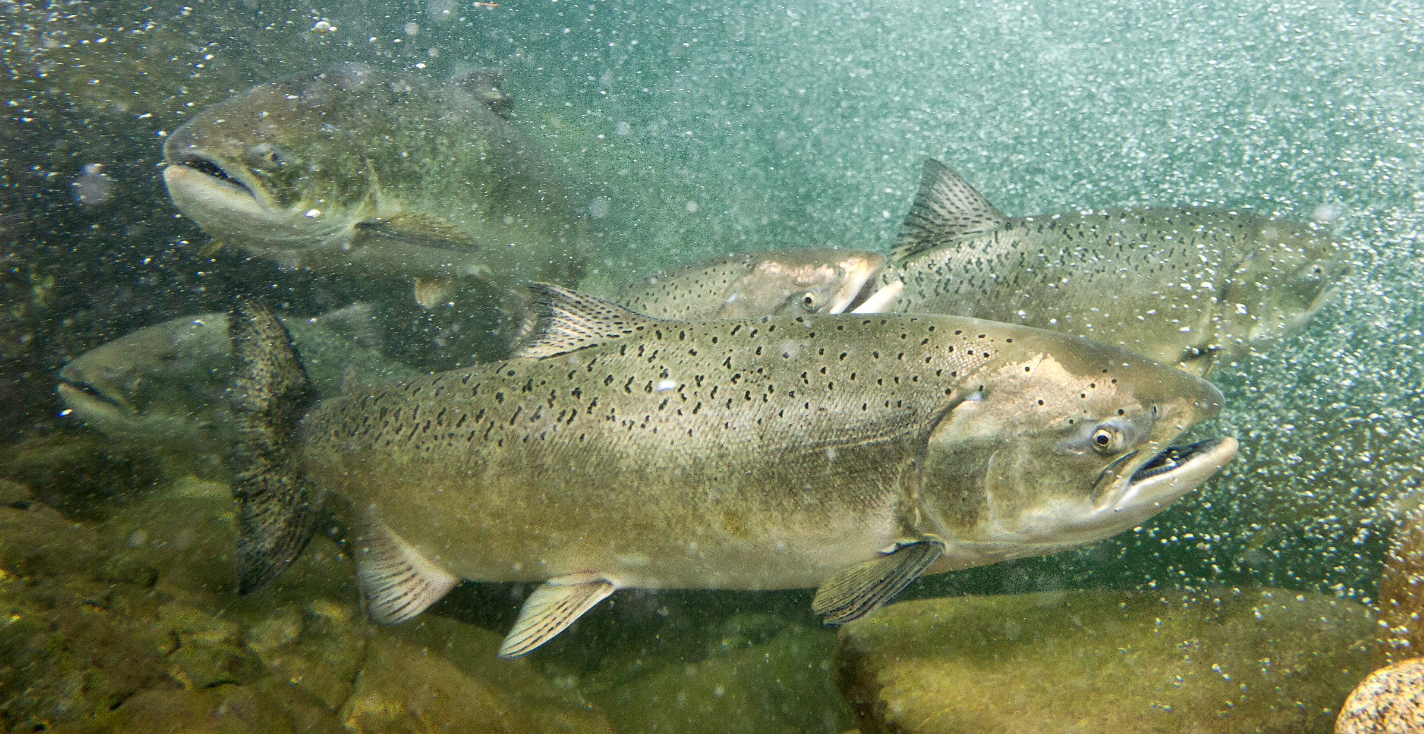
\includegraphics[width=.65\textwidth]{graphics_day2b_popgen/chinook_salmon.png}
	\end{center}
	\caption{The effective population size of the Chinook salmon (\emph{Oncorhynchus tshawytscha}) has been estimated to be very low, possibly because the population size fluctuates between years and high variance in offspring.}
	\end{figure}
	$N_e$ is equal to harmonic mean if sizes fluctuate.\\
	$\to$ Smaller sizes have more impact.
\end{frame}
%%%%%%%%%%%%%%%%%%%%%%%%%%%%%%%%%%%%%%%%%%%%%%%%%%%%%%%%%%%%%%%%%%%%%%%%%%%%%%%%%%%%%%
%
%
%
% %%%%%%%%%%%%%%%%%%%%%%%%%%%%%%%%%%%%%%%%%%%%%%%%%%%%%%%%%%%%%%%%%%%%%%%%%%%%%%%%%%%%%%
% \begin{frame}\frametitle{Effective population size ($N_e$)}
% 	\begin{center}
% 		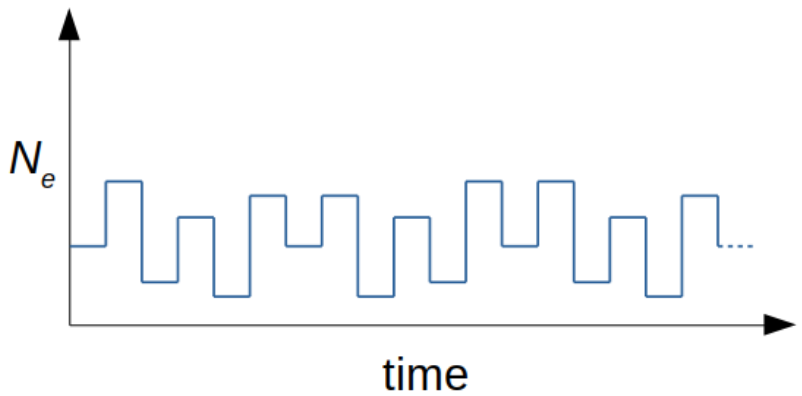
\includegraphics[width=.45\textwidth]{graphics_day2b_popgen/fluctuating_ne.png}
% 	\end{center}
% 	If a population fluctuates between sizes $N_1, N_2, \ldots, N_k$ at a proportion $p_1, p_2, \ldots, p_k$ of the time, the coalescent effective population size is the harmonic mean:
% 	\begin{equation}
% 		N_e = \frac{1}{p_1/N_1 + p_2/N_2 + \ldots + p_k/N_k}
% 	\end{equation}
% 	which is smaller than the arithmetic mean and gives more weight to smaller sizes.
% \end{frame}
% %%%%%%%%%%%%%%%%%%%%%%%%%%%%%%%%%%%%%%%%%%%%%%%%%%%%%%%%%%%%%%%%%%%%%%%%%%%%%%%%%%%%%%
%
%
%
%%%%%%%%%%%%%%%%%%%%%%%%%%%%%%%%%%%%%%%%%%%%%%%%%%%%%%%%%%%%%%%%%%%%%%%%%%%%%%%%%%%%%%
\begin{frame}\frametitle{Effective population size ($N_e$)}
	\begin{center}
		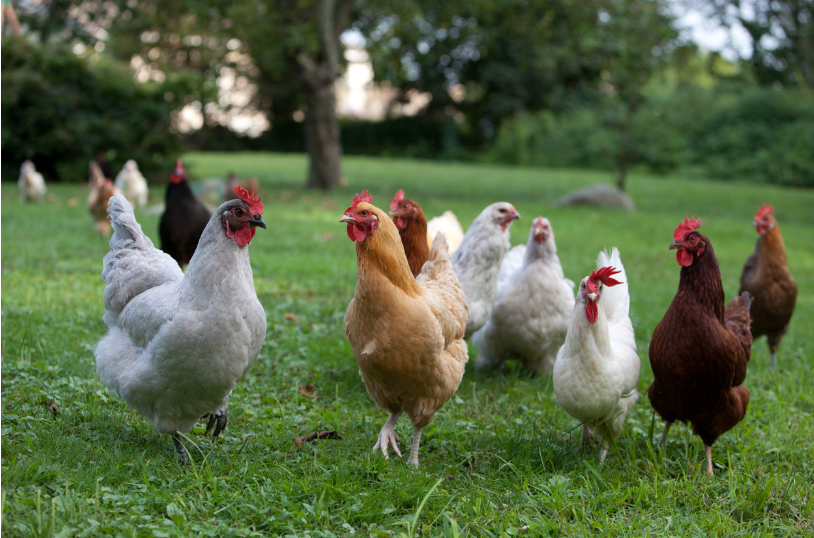
\includegraphics[width=.4\textwidth]{graphics_day2b_popgen/chicken.png}
	\end{center}
	The effective population size with unequal sex ratio is
	\begin{equation}
		N_e = \frac{4N_m N_f}{N_m + N_f}
	\end{equation}
	which is smaller than $N_m + N_f$.
\end{frame}
%%%%%%%%%%%%%%%%%%%%%%%%%%%%%%%%%%%%%%%%%%%%%%%%%%%%%%%%%%%%%%%%%%%%%%%%%%%%%%%%%%%%%%
%
%
%
%%%%%%%%%%%%%%%%%%%%%%%%%%%%%%%%%%%%%%%%%%%%%%%%%%%%%%%%%%%%%%%%%%%%%%%%%%%%%%%%%%%%%%
\begin{frame}\frametitle{Interpreting estimates of $\theta$}
	\begin{center}
		\begin{tabular}{ll}
			\toprule
			\multicolumn{2}{l}{$\pi$ on autosomes}	\\
			\midrule
			Mandenka	& 0.00120	\\
			Biaka		& 0.00121	\\
			San			& 0.00126	\\
			Han			& 0.00081	\\
			Basque		& 0.00087	\\
			Melanesians	& 0.00078	\\
			\bottomrule
	   	\end{tabular}	
	\end{center}
\end{frame}
%%%%%%%%%%%%%%%%%%%%%%%%%%%%%%%%%%%%%%%%%%%%%%%%%%%%%%%%%%%%%%%%%%%%%%%%%%%%%%%%%%%%%%
%
%
%
%%%%%%%%%%%%%%%%%%%%%%%%%%%%%%%%%%%%%%%%%%%%%%%%%%%%%%%%%%%%%%%%%%%%%%%%%%%%%%%%%%%%%%
\begin{frame}\frametitle{Interpreting estimates of $\theta$}
	\begin{center}
		\begin{tabular}{ll}
			\toprule
			\multicolumn{2}{l}{$\pi$ on X chromosomes}	\\
			\midrule
			Mandenka	& 0.00099	\\
			Biaka		& 0.00095	\\
			San			& 0.00085	\\
			Han			& 0.00058	\\
			Basque		& 0.00071	\\
			Melanesians	& 0.00066	\\
			\bottomrule
	   	\end{tabular}	
	\end{center}
\end{frame}
%%%%%%%%%%%%%%%%%%%%%%%%%%%%%%%%%%%%%%%%%%%%%%%%%%%%%%%%%%%%%%%%%%%%%%%%%%%%%%%%%%%%%%
%
%
%
%%%%%%%%%%%%%%%%%%%%%%%%%%%%%%%%%%%%%%%%%%%%%%%%%%%%%%%%%%%%%%%%%%%%%%%%%%%%%%%%%%%%%%
\begin{frame}\frametitle{Summary statistics}
	Possible summaries of DNA sequence data are:
	\begin{itemize}
		\item The number of segregating sites ($S$).
		\item The average number of pairwise differences ($\pi$).
	\end{itemize}
	but they do not provide much information regarding \textbf{allele frequencies}.
\end{frame}
%%%%%%%%%%%%%%%%%%%%%%%%%%%%%%%%%%%%%%%%%%%%%%%%%%%%%%%%%%%%%%%%%%%%%%%%%%%%%%%%%%%%%%
%
%
%
%%%%%%%%%%%%%%%%%%%%%%%%%%%%%%%%%%%%%%%%%%%%%%%%%%%%%%%%%%%%%%%%%%%%%%%%%%%%%%%%%%%%%%
\begin{frame}\frametitle{The Site Frequency Spectrum (SFS)}
	\begin{block}{SFS}
		The SFS is obtained by tabulating the sample allele frequencies of all mutations.
	\end{block}
	\begin{columns}
	\begin{column}{0.25\textwidth}
	\begin{center}
		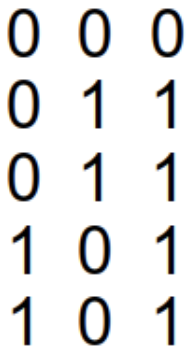
\includegraphics[width=.42\textwidth]{graphics_day2b_popgen/small_ims_matrix.png}
	\end{center}
	\end{column}
	\begin{column}{0.75\textwidth}
\visible<2-3>{$~$\\[1ex]The ``1'' alleles have frequencies 2/5, 2/5 and 4/5. The proportions of ``1'' alleles with a frequency of\\ 1/5, 2/5, 3/5 and 4/5 in the sample are\\
\visible<3>{$f_1 = 0$, $f_2 =2/3$, $f_3 = 0$ and $f_4 =1/3$.
		\begin{equation}
			\vec{f} = (f_1, f_2, \ldots, f_{n-1})
		\end{equation}
		for a sample of $n$ haploid individuals.}}
	\end{column}
	\end{columns}
\end{frame}
%%%%%%%%%%%%%%%%%%%%%%%%%%%%%%%%%%%%%%%%%%%%%%%%%%%%%%%%%%%%%%%%%%%%%%%%%%%%%%%%%%%%%%
%
%
%
%%%%%%%%%%%%%%%%%%%%%%%%%%%%%%%%%%%%%%%%%%%%%%%%%%%%%%%%%%%%%%%%%%%%%%%%%%%%%%%%%%%%%%
\begin{frame}\frametitle{The Site Frequency Spectrum (SFS)}
	\begin{columns}
	\begin{column}{0.25\textwidth}
		\begin{center}
			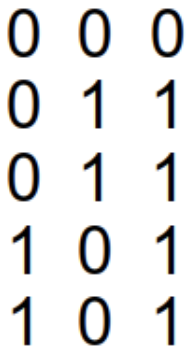
\includegraphics[width=.42\textwidth]{graphics_day2b_popgen/small_ims_matrix.png}
		\end{center}
	\end{column}
	\begin{column}{0.75\textwidth}
		\begin{center}
			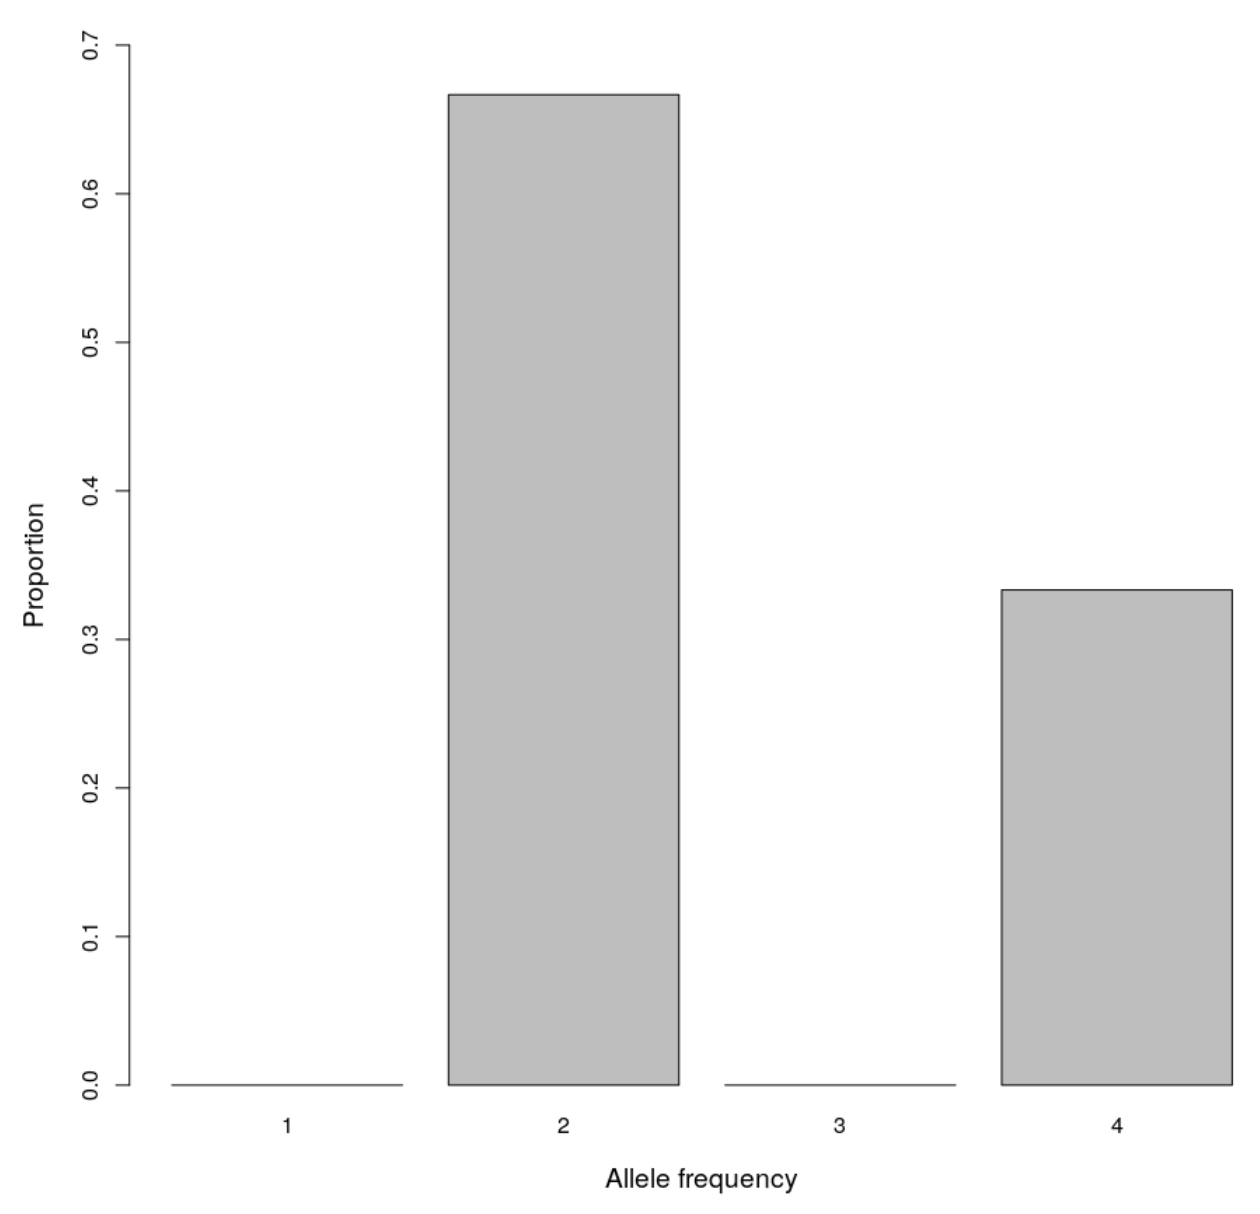
\includegraphics[width=.85\textwidth]{graphics_day2b_popgen/sfs_plot.png}
		\end{center}
	\end{column}
	\end{columns}
\end{frame}
%%%%%%%%%%%%%%%%%%%%%%%%%%%%%%%%%%%%%%%%%%%%%%%%%%%%%%%%%%%%%%%%%%%%%%%%%%%%%%%%%%%%%%
%
%
%
%%%%%%%%%%%%%%%%%%%%%%%%%%%%%%%%%%%%%%%%%%%%%%%%%%%%%%%%%%%%%%%%%%%%%%%%%%%%%%%%%%%%%%
\begin{frame}\frametitle{Alleles}
	\begin{itemize}
		\item \textbf{Ancestral} allele is the allele found in the MRCA of the sample.
		\item \textbf{Derived} allele (or mutated) is an allele that is not ancestral.
	\end{itemize}
	\begin{center}
		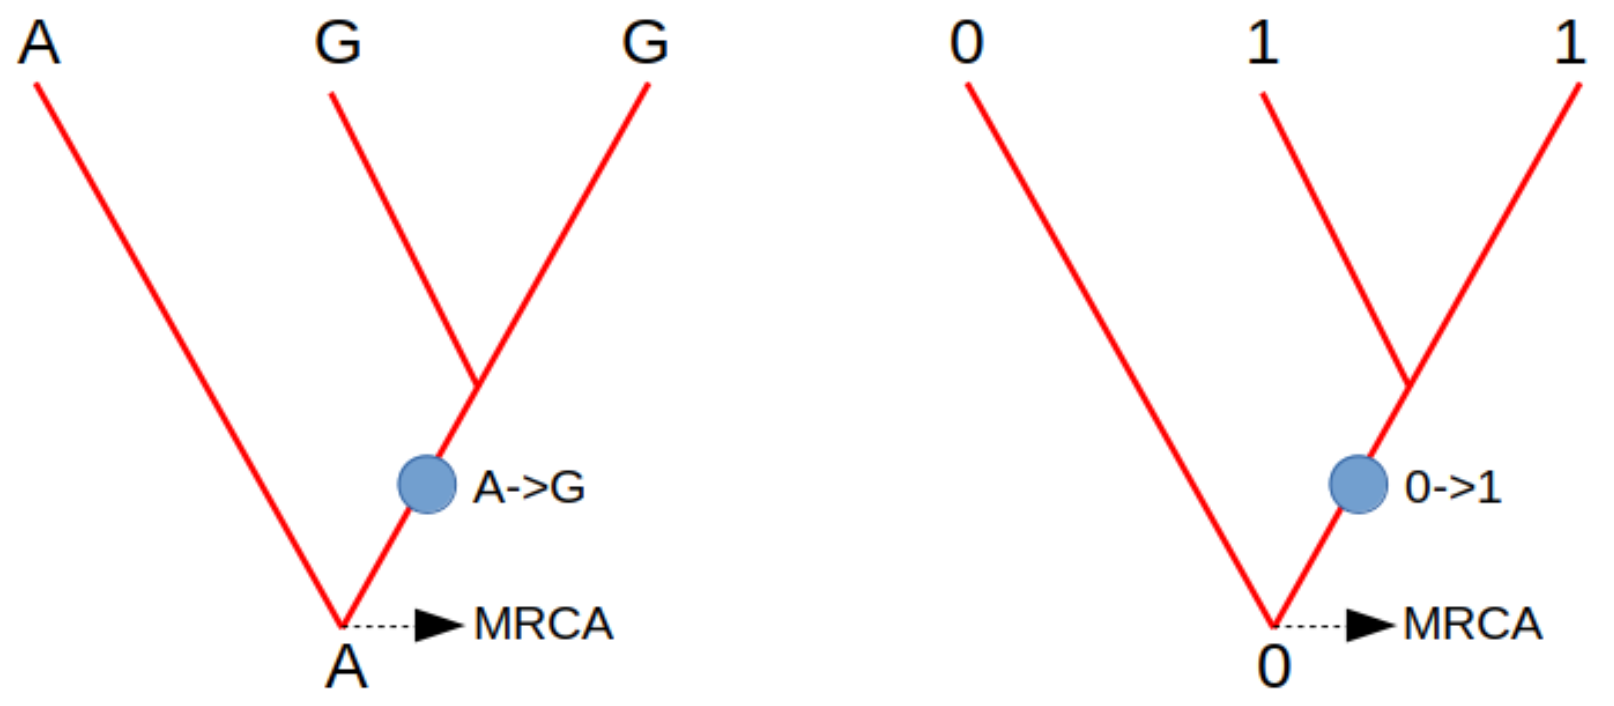
\includegraphics[width=.8\textwidth]{graphics_day2b_popgen/ancestral_allele.png}
	\end{center}
\end{frame}
%%%%%%%%%%%%%%%%%%%%%%%%%%%%%%%%%%%%%%%%%%%%%%%%%%%%%%%%%%%%%%%%%%%%%%%%%%%%%%%%%%%%%%
%
%
%
%%%%%%%%%%%%%%%%%%%%%%%%%%%%%%%%%%%%%%%%%%%%%%%%%%%%%%%%%%%%%%%%%%%%%%%%%%%%%%%%%%%%%%
\begin{frame}\frametitle{Alleles}
	The ancestral allele is often inferred using \textbf{outgroups}.\\
	E.g.\ if \texttt{C/T} polymorphism in humans and primate have \texttt{C}, then \texttt{C} is likely to be the ancestral allele.
	\begin{center}
		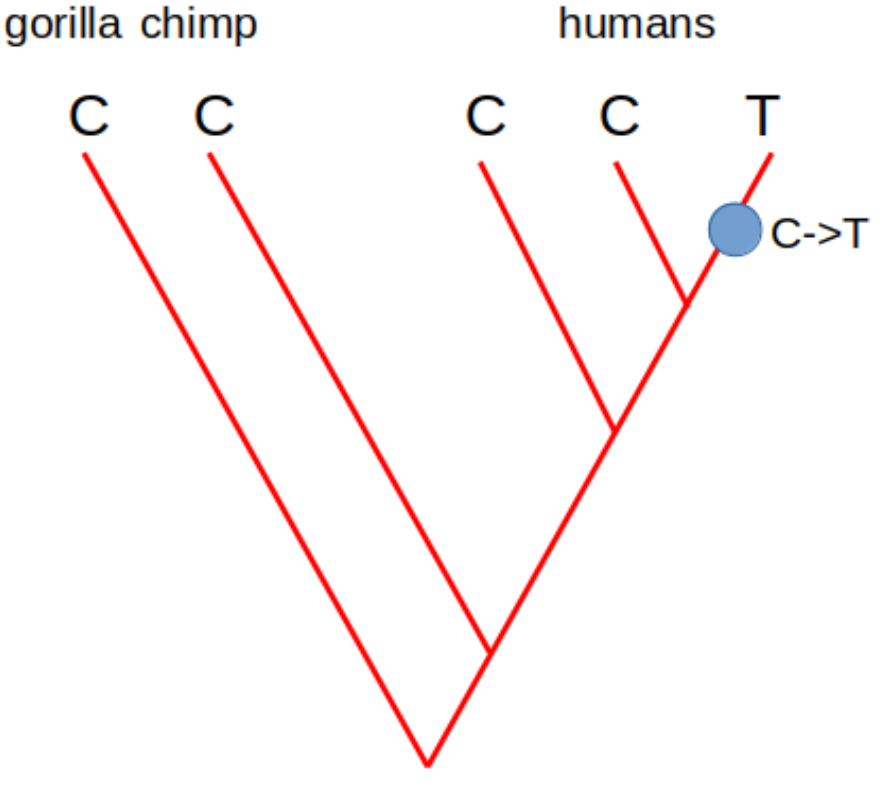
\includegraphics[width=.45\textwidth]{graphics_day2b_popgen/allele_outgroup.png}
	\end{center}
	$\to$ Folded SFS if ancestral/derived informatio not available.
\end{frame}
%%%%%%%%%%%%%%%%%%%%%%%%%%%%%%%%%%%%%%%%%%%%%%%%%%%%%%%%%%%%%%%%%%%%%%%%%%%%%%%%%%%%%%
%
%
%
%%%%%%%%%%%%%%%%%%%%%%%%%%%%%%%%%%%%%%%%%%%%%%%%%%%%%%%%%%%%%%%%%%%%%%%%%%%%%%%%%%%%%%
\begin{frame}\frametitle{The Site Frequency Spectrum}
	\begin{itemize}
		\item $S$ and $\pi$ can be calculated directly from $\vec{f}$ but the opposite is not true.
		\item Alleles segregating at frequency of 1/n are called \textbf{singletons}.
		\item The expected SFS under the standard coalescence model with
infinite sites mutations is
			\begin{equation}
				\E[f_i] = \frac{1/i}{\sum_{k=1}^{n-1}\tfrac{1}{k}}
			\end{equation}
			with $i = 1,2,\ldots,n-1$.
	\end{itemize}
\end{frame}
%%%%%%%%%%%%%%%%%%%%%%%%%%%%%%%%%%%%%%%%%%%%%%%%%%%%%%%%%%%%%%%%%%%%%%%%%%%%%%%%%%%%%%
%
%
%
%%%%%%%%%%%%%%%%%%%%%%%%%%%%%%%%%%%%%%%%%%%%%%%%%%%%%%%%%%%%%%%%%%%%%%%%%%%%%%%%%%%%%%
\begin{frame}\frametitle{Expected Site Frequency Spectrum}
	\begin{figure}
	\begin{center}
		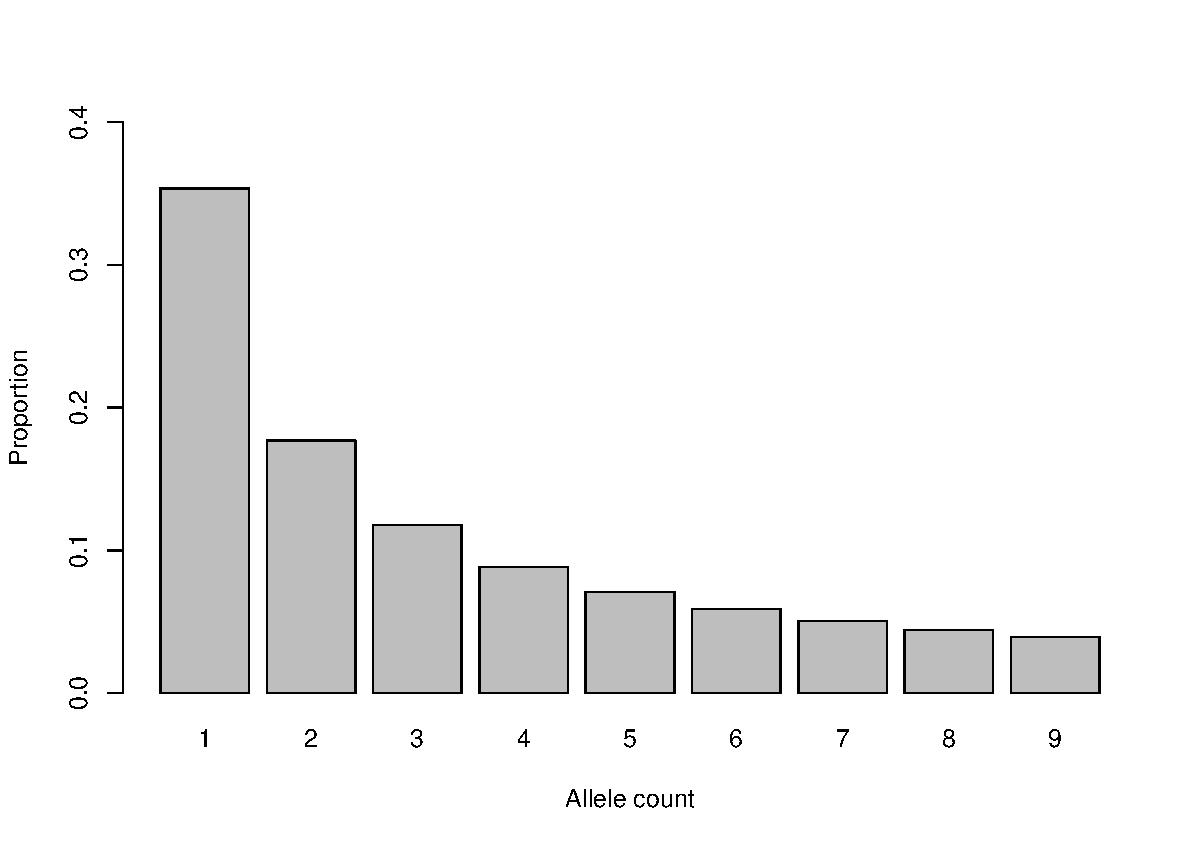
\includegraphics[width=.55\textwidth]{graphics_day2b_popgen/sfs.pdf}
	\end{center}
	\caption{The expected SFS for $n=10$.}
	\end{figure}
\end{frame}
%%%%%%%%%%%%%%%%%%%%%%%%%%%%%%%%%%%%%%%%%%%%%%%%%%%%%%%%%%%%%%%%%%%%%%%%%%%%%%%%%%%%%%
%
%
%
% %%%%%%%%%%%%%%%%%%%%%%%%%%%%%%%%%%%%%%%%%%%%%%%%%%%%%%%%%%%%%%%%%%%%%%%%%%%%%%%%%%%%%%
% \begin{frame}\frametitle{Alleles}
% 	\begin{figure}
% 	\begin{center}
% 		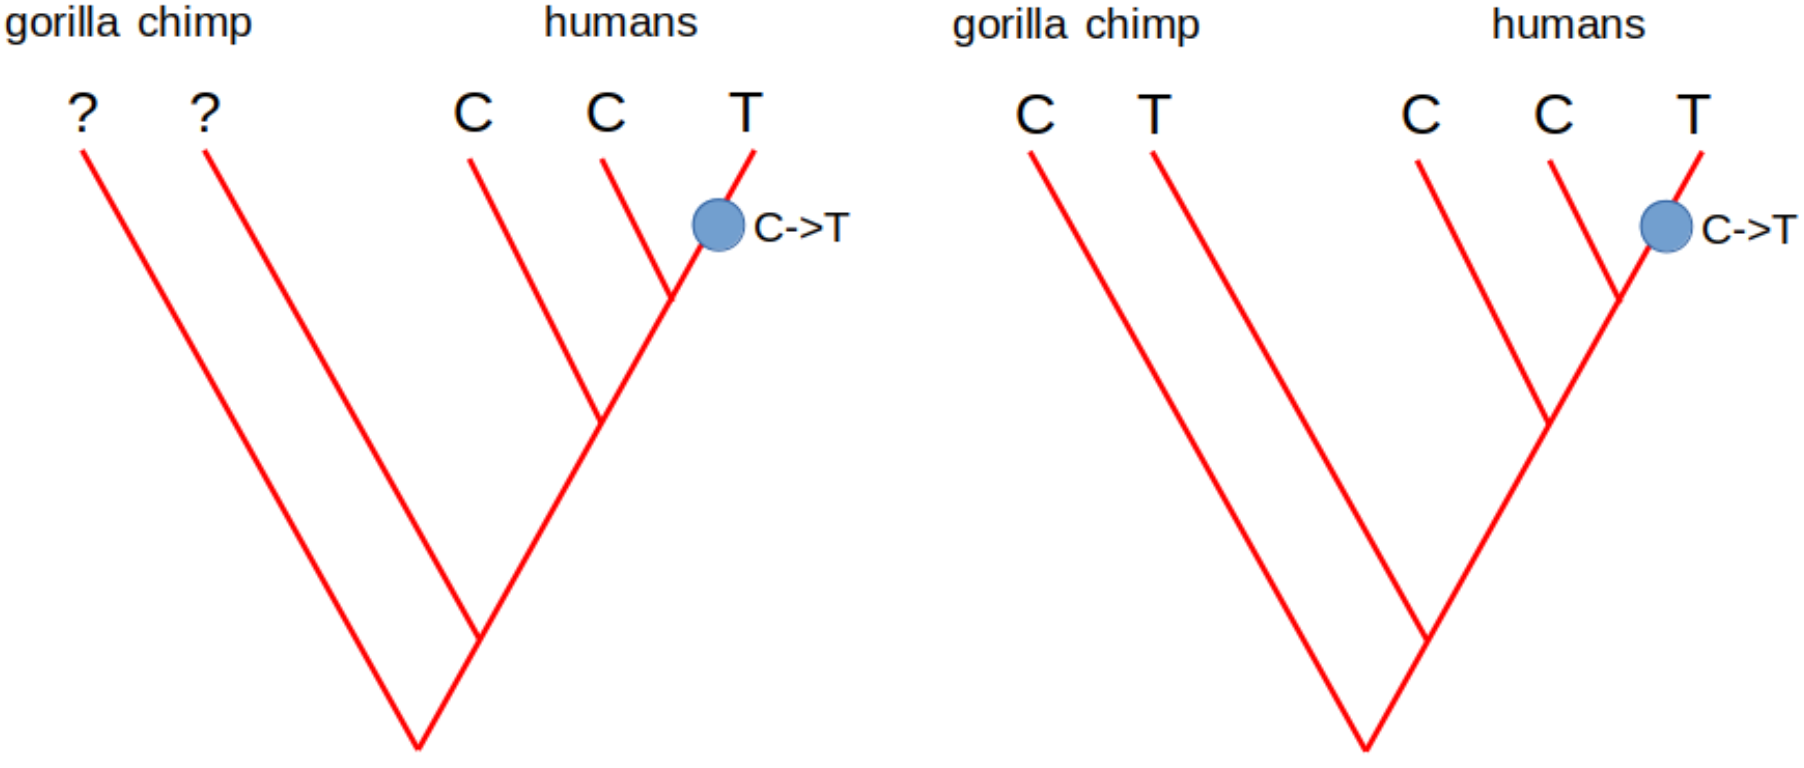
\includegraphics[width=.8\textwidth]{graphics_day2b_popgen/allele_outgroup_uncertain.png}
% 	\end{center}
% 	\caption{Uncertain ancestral allele.}
% 	\end{figure}
% \end{frame}
% %%%%%%%%%%%%%%%%%%%%%%%%%%%%%%%%%%%%%%%%%%%%%%%%%%%%%%%%%%%%%%%%%%%%%%%%%%%%%%%%%%%%%%
% %
% %
% %
% %%%%%%%%%%%%%%%%%%%%%%%%%%%%%%%%%%%%%%%%%%%%%%%%%%%%%%%%%%%%%%%%%%%%%%%%%%%%%%%%%%%%%%
% \begin{frame}\frametitle{The Site Frequency Spectrum (SFS)}
% 	If no information on the ancestral allele is available, we can fold the frequency spectrum.
% 	\begin{block}{}
% 		The \textbf{folded frequency spectrum} $f^*$ is obtained by adding together the frequencies of the derived and ancestral alleles.
% 	\end{block}
% 	$f^*_j = f_j+f_{n-j}$ for $j<n/2$ and\\
% 	$f^*_j = f_j$ for $j=n/2$\\
% 	only defined for values of $f^*_j \leq n/2$.
% \end{frame}
% %%%%%%%%%%%%%%%%%%%%%%%%%%%%%%%%%%%%%%%%%%%%%%%%%%%%%%%%%%%%%%%%%%%%%%%%%%%%%%%%%%%%%%
% %
% %
% %
% %%%%%%%%%%%%%%%%%%%%%%%%%%%%%%%%%%%%%%%%%%%%%%%%%%%%%%%%%%%%%%%%%%%%%%%%%%%%%%%%%%%%%%
% \begin{frame}\frametitle{The folded SFS}
% 	\begin{columns}
% 	\begin{column}{0.25\textwidth}
% 	\begin{center}
% 		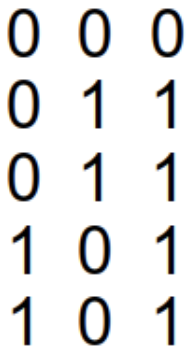
\includegraphics[width=.42\textwidth]{graphics_day2b_popgen/small_ims_matrix.png}
% 	\end{center}
% 	\end{column}
% 	\begin{column}{0.75\textwidth}
% 		\begin{equation}
% 			\begin{split}
% 				\vec{f} & = (f_1=0, f_2=2/3, f_3=0, f_4=1/3)\\
% 				\vec{f^*} & = \visible<2>{(f_1^* = 1/3, f_2^* = 2/3)}\\
% 			\end{split}
% 		\end{equation}
% 	\end{column}
% 	\end{columns}
% \end{frame}
% %%%%%%%%%%%%%%%%%%%%%%%%%%%%%%%%%%%%%%%%%%%%%%%%%%%%%%%%%%%%%%%%%%%%%%%%%%%%%%%%%%%%%%
% %
% %
% %
% %%%%%%%%%%%%%%%%%%%%%%%%%%%%%%%%%%%%%%%%%%%%%%%%%%%%%%%%%%%%%%%%%%%%%%%%%%%%%%%%%%%%%%
% \begin{frame}\frametitle{Expected folded SFS}
% 	\begin{figure}
% 	\begin{center}
% 		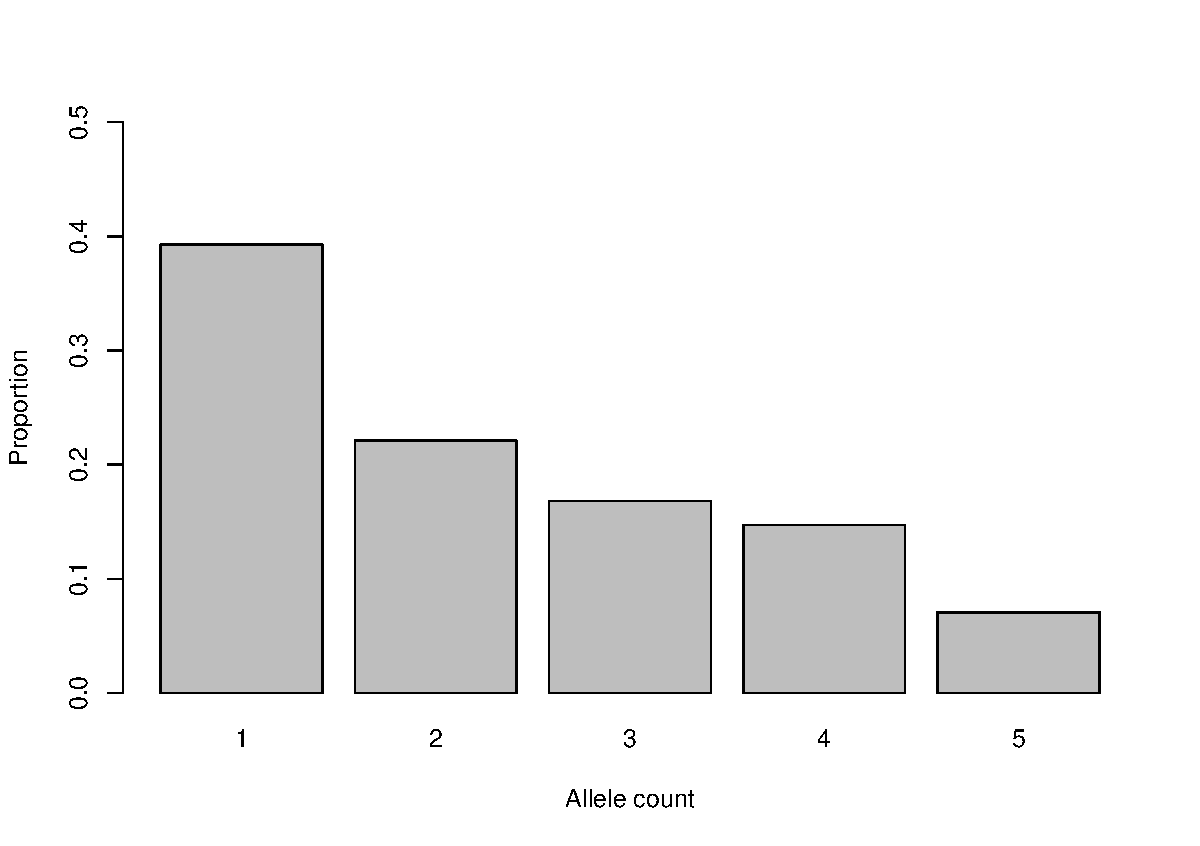
\includegraphics[width=.55\textwidth]{graphics_day2b_popgen/folded_sfs.pdf}
% 	\end{center}
% 	\caption{The expected folded SFS for $n=10$.}
% 	\end{figure}
% \end{frame}
% %%%%%%%%%%%%%%%%%%%%%%%%%%%%%%%%%%%%%%%%%%%%%%%%%%%%%%%%%%%%%%%%%%%%%%%%%%%%%%%%%%%%%%
%
%
%
%%%%%%%%%%%%%%%%%%%%%%%%%%%%%%%%%%%%%%%%%%%%%%%%%%%%%%%%%%%%%%%%%%%%%%%%%%%%%%%%%%%%%%
\begin{frame}\frametitle{Tree shape and population size}
	Measured in number of generations, the expected coalescence time for $k$ lineages is $2N/[k(k - 1)]$.
	\begin{center}
\only<1>{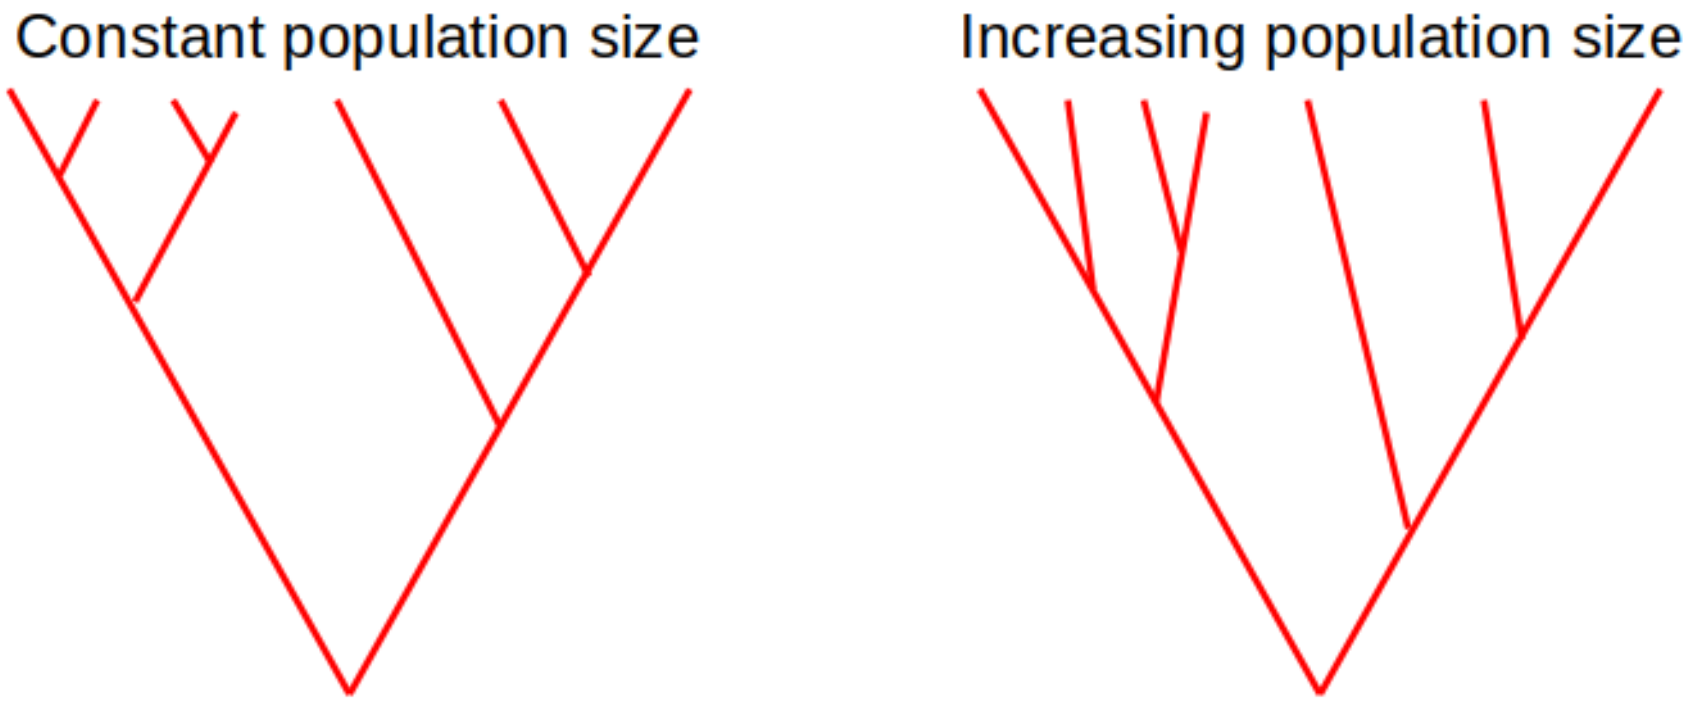
\includegraphics[width=.8\textwidth]{graphics_day2b_popgen/trees_ne_increasing.png}}
\only<2>{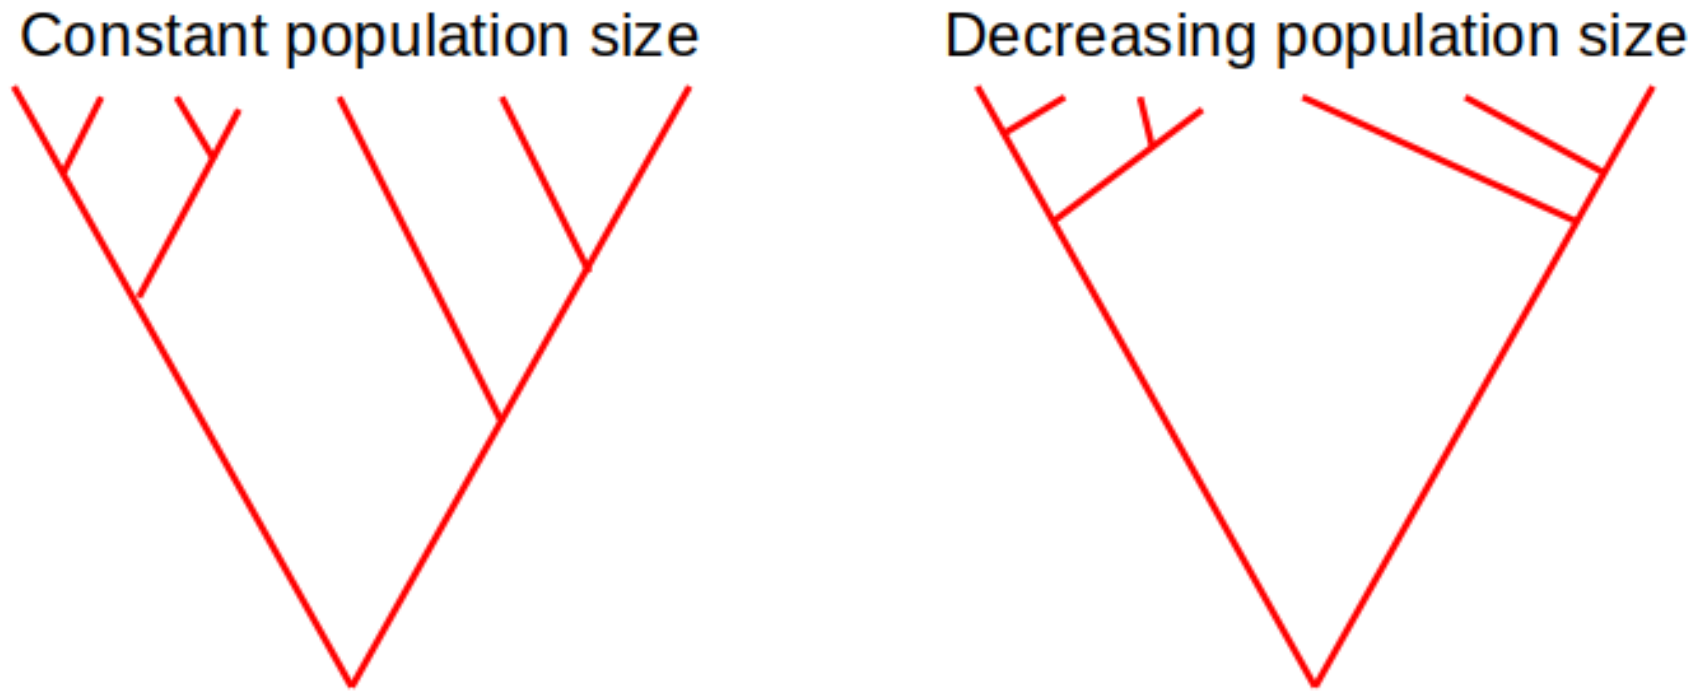
\includegraphics[width=.8\textwidth]{graphics_day2b_popgen/trees_ne_decreasing.png}}
	\end{center}
\end{frame}
%%%%%%%%%%%%%%%%%%%%%%%%%%%%%%%%%%%%%%%%%%%%%%%%%%%%%%%%%%%%%%%%%%%%%%%%%%%%%%%%%%%%%%
%
%
%
%%%%%%%%%%%%%%%%%%%%%%%%%%%%%%%%%%%%%%%%%%%%%%%%%%%%%%%%%%%%%%%%%%%%%%%%%%%%%%%%%%%%%%
\begin{frame}\frametitle{Intended Learning Outcomes}
	\textbf{Coalescent theory}\\[2ex]
	In this lecture you have learnt to
	\begin{itemize}
		\item Describe principles and assumptions of the coalescence theory.
		\item Discuss the infinite sites model.
		\item Provide estimators of $\theta$ and effective population sizes.
		\item Measure genetic variability with summary statistics and the site frequency spectrum.
	\end{itemize}
\end{frame}
%%%%%%%%%%%%%%%%%%%%%%%%%%%%%%%%%%%%%%%%%%%%%%%%%%%%%%%%%%%%%%%%%%%%%%%%%%%%%%%%%%%%%%
%
%
%
%%%%%%%%%%%%%%%%%%%%%%%%%%%%%%%%%%%%%%%%%%%%%%%%%%%%%%%%%%%%%%%%%%%%%%%%%%%%%%%%%%%%%%
\begin{frame}\frametitle{Intended Learning Outcomes}
	\textbf{Population subdivision}\\[2ex]
	In this lecture you will learn to
	\begin{itemize}
		\item Quantify the effect of population subdivision on allele frequencies and heterozygosity.
		\item Calculate measures of population genetic differentiation.
		\item Discuss divergence models.
	\end{itemize}
\end{frame}
%%%%%%%%%%%%%%%%%%%%%%%%%%%%%%%%%%%%%%%%%%%%%%%%%%%%%%%%%%%%%%%%%%%%%%%%%%%%%%%%%%%%%%
%
%
%
%%%%%%%%%%%%%%%%%%%%%%%%%%%%%%%%%%%%%%%%%%%%%%%%%%%%%%%%%%%%%%%%%%%%%%%%%%%%%%%%%%%%%%
\begin{frame}\frametitle{Population subdivision}
	\begin{block}{}
		There is population subdivision, or \textbf{structure}, when the population is not randomly mating because of geographic or social structure.
	\end{block}
	Population subdivision is important to
	\begin{itemize}
		\item Understand the effects of drift and natural selection.
		\item Plan conservation strategies for rare or endangered species.
	\end{itemize}
\end{frame}
%%%%%%%%%%%%%%%%%%%%%%%%%%%%%%%%%%%%%%%%%%%%%%%%%%%%%%%%%%%%%%%%%%%%%%%%%%%%%%%%%%%%%%
%
%
%
%%%%%%%%%%%%%%%%%%%%%%%%%%%%%%%%%%%%%%%%%%%%%%%%%%%%%%%%%%%%%%%%%%%%%%%%%%%%%%%%%%%%%%
\begin{frame}\frametitle{Population subdivision}
	\begin{center}
\only<1>{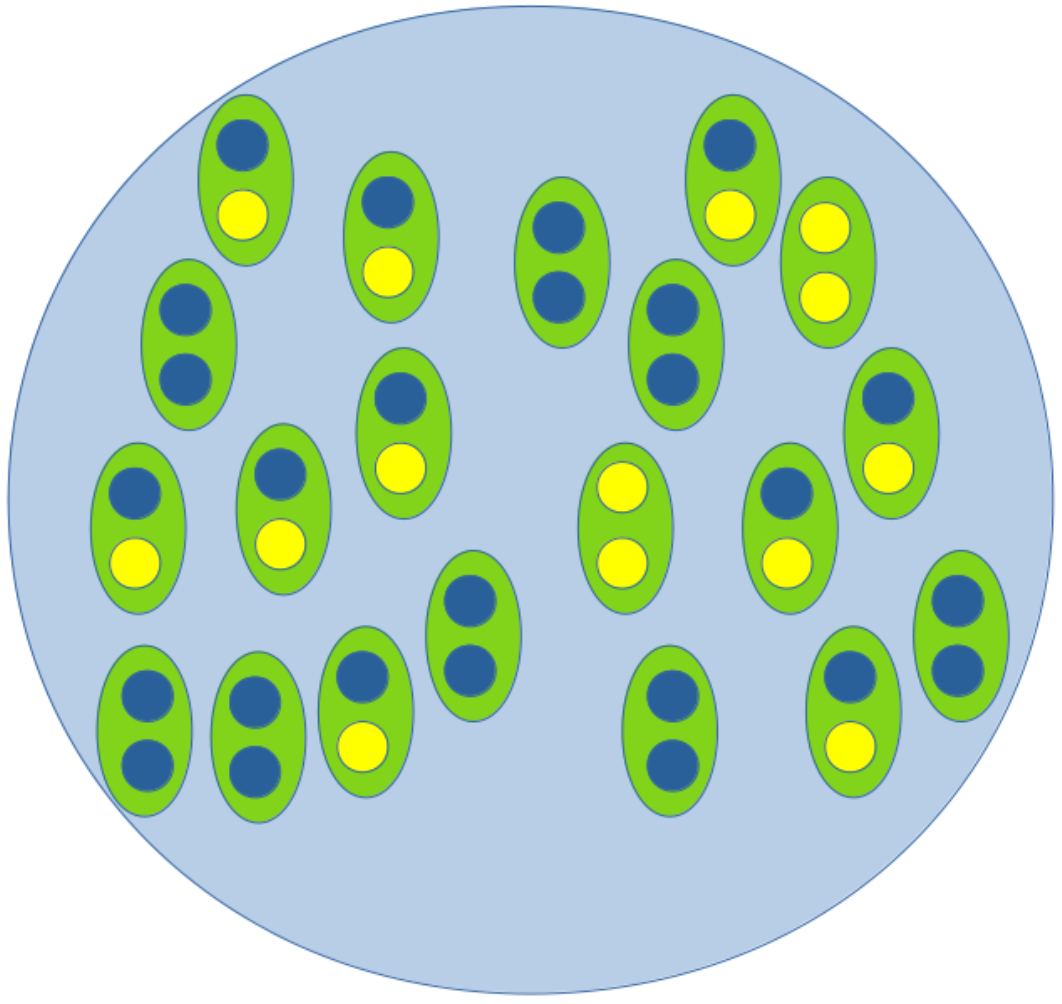
\includegraphics[width=.5\textwidth]{graphics_day2b_popgen/structure_panmictic.png}}
\only<2>{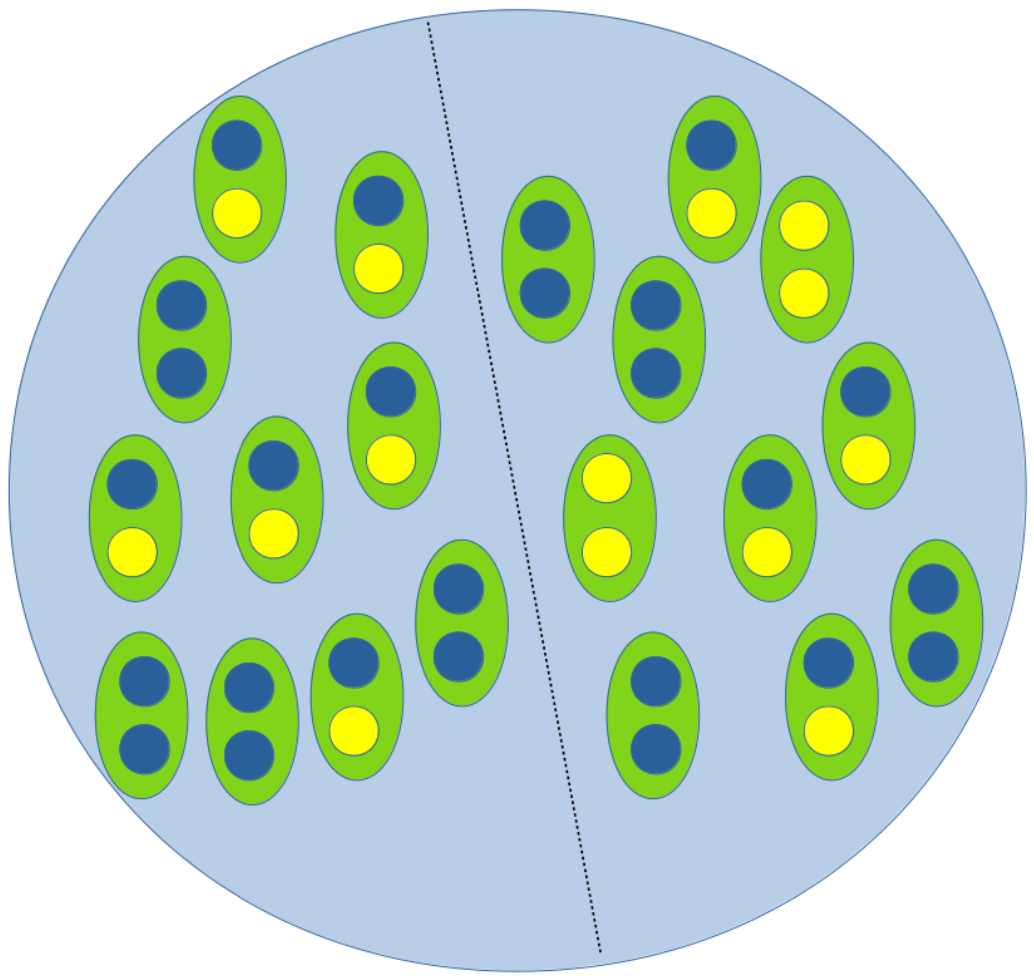
\includegraphics[width=.5\textwidth]{graphics_day2b_popgen/structure_divided.png}}
	\end{center}
\end{frame}
%%%%%%%%%%%%%%%%%%%%%%%%%%%%%%%%%%%%%%%%%%%%%%%%%%%%%%%%%%%%%%%%%%%%%%%%%%%%%%%%%%%%%%
%
%
%
%%%%%%%%%%%%%%%%%%%%%%%%%%%%%%%%%%%%%%%%%%%%%%%%%%%%%%%%%%%%%%%%%%%%%%%%%%%%%%%%%%%%%%
\begin{frame}\frametitle{Allele frequencies in a subdivided population}
	\begin{columns}
	\begin{column}{0.33\textwidth}
		\begin{center}
			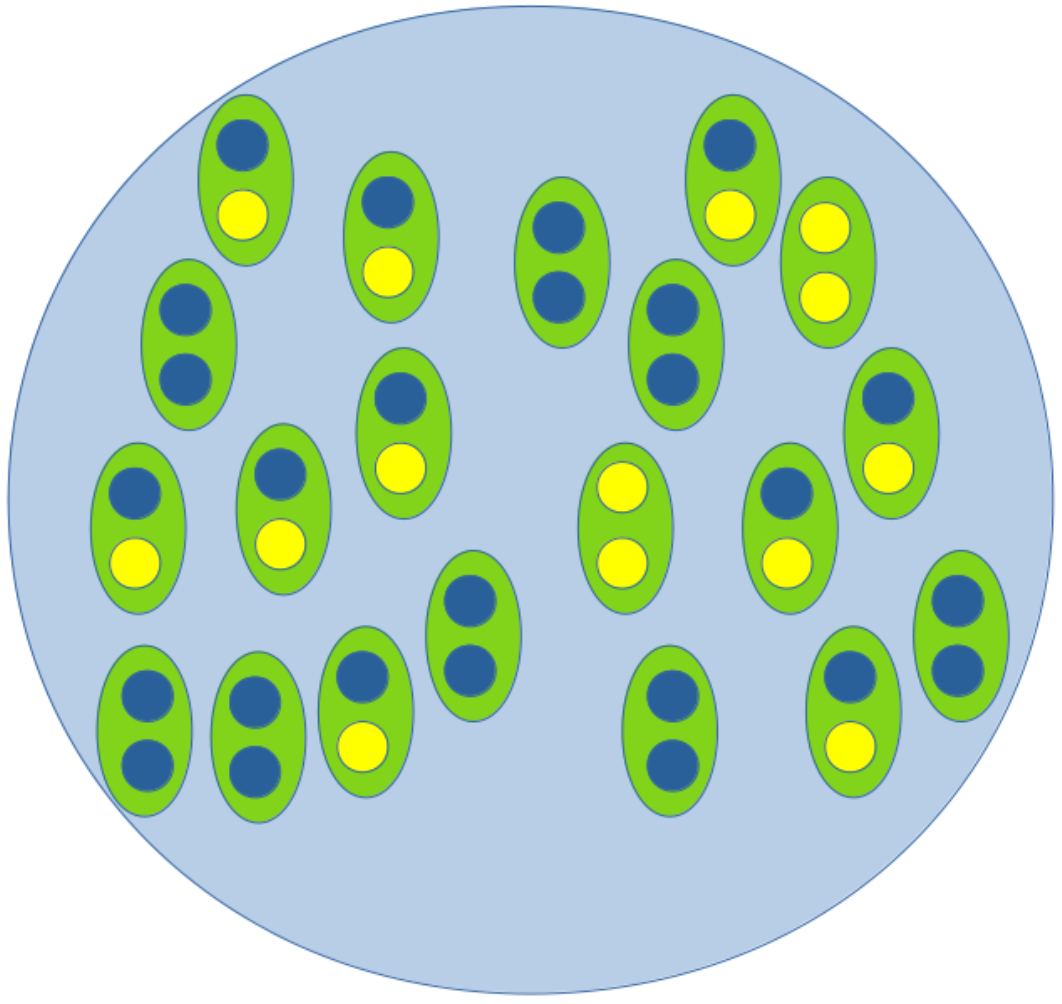
\includegraphics[width=.7\textwidth]{graphics_day2b_popgen/structure_panmictic.png}\\[2ex]
			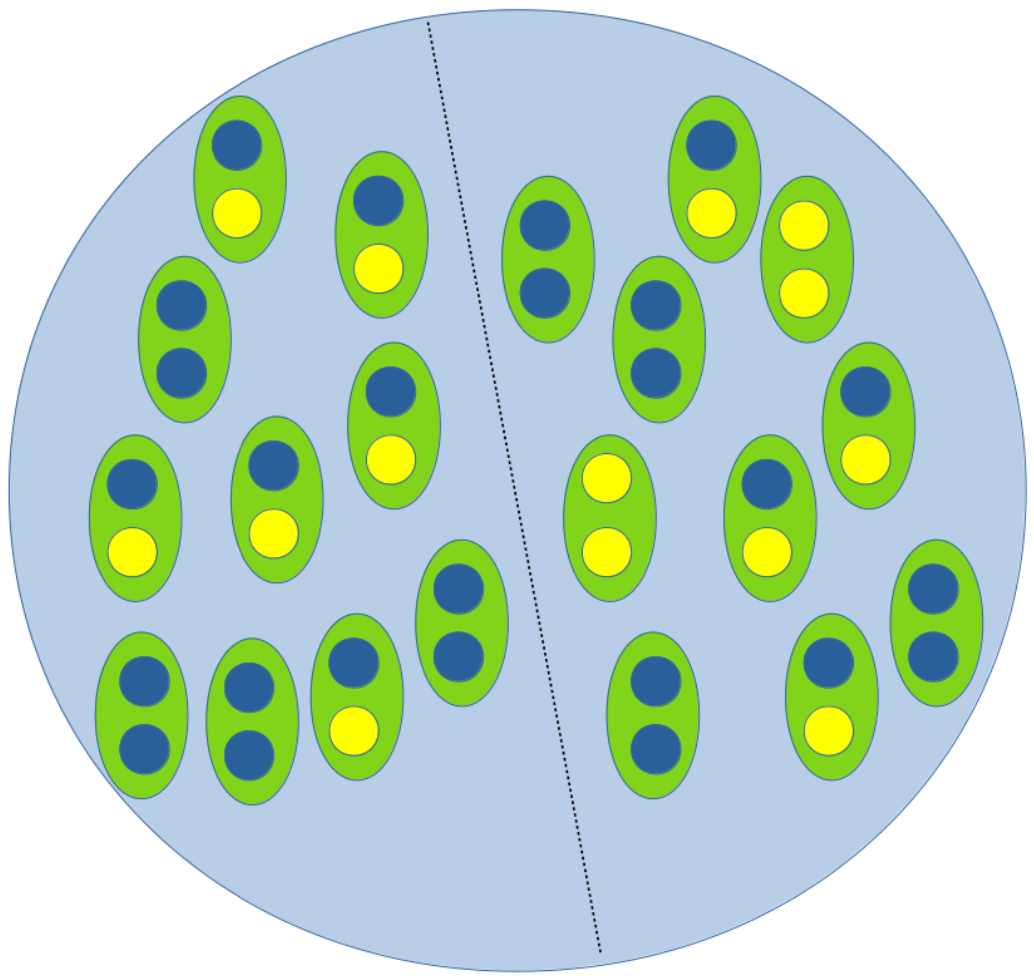
\includegraphics[width=.7\textwidth]{graphics_day2b_popgen/structure_divided.png}
		\end{center}
	\end{column}
	\begin{column}{0.66\textwidth}
\only<1>{Assume two subpopulations, each one in HWE with $N_1$ and $N_2$ individuals, respectively.\\[1.5ex]
		The average frequency of allele $A$ when pooling the two subpopulations is
		\begin{equation}
			f_A = \frac{2N_1 f_{A1} + 2N_2 f_{A2}}{2N_1 + 2N_2}
		\end{equation}
		if $N_1 = N_2$
		\begin{equation}
			f_A = \frac{f_{A1} + f_{A2}}{2}
		\end{equation}}%
\only<2>{The proportion of heterozygous individuals is
		\begin{equation}
			H_S = \frac{2f_{A1}(1-f_{A1}) + 2f_{A2}(1-f_{A2})}{2}
		\end{equation}
		which is the expected heterozygosity when both populations are sampled.\\[1.5ex]
		$S$ in $H_S$ stands for ``in the subdivided population''}%
\only<3>{However, the expected proportion of heterozygous individuals in a population with frequency $f_A$ is
		\begin{equation}
			H_T = 2\frac{f_{A1}+f_{A2}}{2}\Big( 1 - \frac{f_{A1}+f_{A2}}{2}\Big)
		\end{equation}
		$T$ in $H_T$ stands for ``in the total (pooled) population''}%
	\end{column}
	\end{columns}
\end{frame}
%%%%%%%%%%%%%%%%%%%%%%%%%%%%%%%%%%%%%%%%%%%%%%%%%%%%%%%%%%%%%%%%%%%%%%%%%%%%%%%%%%%%%%
%
%
%
%%%%%%%%%%%%%%%%%%%%%%%%%%%%%%%%%%%%%%%%%%%%%%%%%%%%%%%%%%%%%%%%%%%%%%%%%%%%%%%%%%%%%%
\begin{frame}\frametitle{Heterozygosity in a subdivided population}
	After some rearrangements we have
	\begin{equation}
		H_S = f_{A1}(1-f_{A1}) + f_{A2}(1-f_{A2})
	\end{equation}
	and
	\begin{equation}
		H_T = f_{A1}(1-f_{A1}) + f_{A2}(1-f_{A2}) + \delta^2/2
	\end{equation}
	with $\delta = |f_{A1} - f_{A2}|$.
\end{frame}
%%%%%%%%%%%%%%%%%%%%%%%%%%%%%%%%%%%%%%%%%%%%%%%%%%%%%%%%%%%%%%%%%%%%%%%%%%%%%%%%%%%%%%
%
%
%%%%%%%%%%%%%%%%%%%%%%%%%%%%%%%%%%%%%%%%%%%%%%%%%%%%%%%%%%%%%%%%%%%%%%%%%%%%%%%%%%%%%%%
\begin{frame}\frametitle{Heterozygosity in a subdivided population}
	\begin{equation}
		H_T = H_S + \delta^2/2
	\end{equation}
	\begin{itemize}
		\item If $\delta = 0$ then \visible<2-4>{$H_T = H_S$ and the total (pooled) population is also in HWE.}
		\item \visible<2-4>{If $\delta >> 0$ then \visible<3-4>{$H_T > H_S$ and \visible<4>{the total (pooled) population contains fewer heterozygous individuals than expected given the pooled allele frequency.}}}
	\end{itemize}
\visible<4>{\begin{block}{Wahlund effect}
		The decrease of heterozygosity in a subdivided population compared to a randomly mating one with the same (total) allele frequency.
	\end{block}}
\end{frame}
%%%%%%%%%%%%%%%%%%%%%%%%%%%%%%%%%%%%%%%%%%%%%%%%%%%%%%%%%%%%%%%%%%%%%%%%%%%%%%%%%%%%%%
%
%
%
%%%%%%%%%%%%%%%%%%%%%%%%%%%%%%%%%%%%%%%%%%%%%%%%%%%%%%%%%%%%%%%%%%%%%%%%%%%%%%%%%%%%%%%
\begin{frame}\frametitle{Quantifying population subdivision}
	\begin{equation}
		F_{ST} = \frac{H_T - H_S}{H_T}
	\end{equation}
\only<2>{$F_{ST}$ has a range defined as
	\begin{itemize}
		\item If $\delta=0$ then $H_1T = H_S$ and $F_{ST} =0$.
		\item If $\delta >> 0$ then $F_{ST} \approx 1$.
	\end{itemize}
	$F_{ST}$ can be calculated for more than two subpopulations.}
\end{frame}
%%%%%%%%%%%%%%%%%%%%%%%%%%%%%%%%%%%%%%%%%%%%%%%%%%%%%%%%%%%%%%%%%%%%%%%%%%%%%%%%%%%%%%
%
%
%
%%%%%%%%%%%%%%%%%%%%%%%%%%%%%%%%%%%%%%%%%%%%%%%%%%%%%%%%%%%%%%%%%%%%%%%%%%%%%%%%%%%%%%%
\begin{frame}\frametitle{$F_{ST}$: population genetic differentiation}
	\begin{figure}
	\begin{center}
		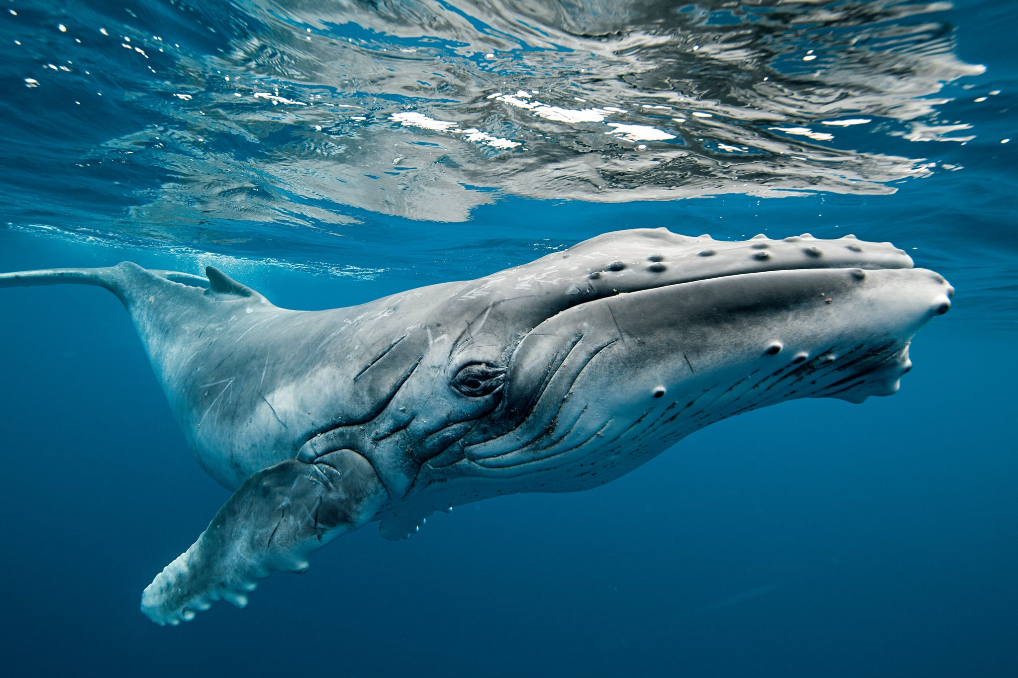
\includegraphics[width=.55\textwidth]{graphics_day2b_popgen/humpback_whale.png}
	\end{center}
	\caption{Humpback whales in the Pacific and Atlantic have strong genetic differentiation ($F_{ST} > 0.4$) while populations in the North Atlantic have low differentation ($F_{ST} \approx 0.04$).}
	\end{figure}
\end{frame}
%%%%%%%%%%%%%%%%%%%%%%%%%%%%%%%%%%%%%%%%%%%%%%%%%%%%%%%%%%%%%%%%%%%%%%%%%%%%%%%%%%%%%%
%
%
%
%%%%%%%%%%%%%%%%%%%%%%%%%%%%%%%%%%%%%%%%%%%%%%%%%%%%%%%%%%%%%%%%%%%%%%%%%%%%%%%%%%%%%%%
\begin{frame}\frametitle{Wright-Fisher model with migration}
	\begin{figure}
	\begin{center}
		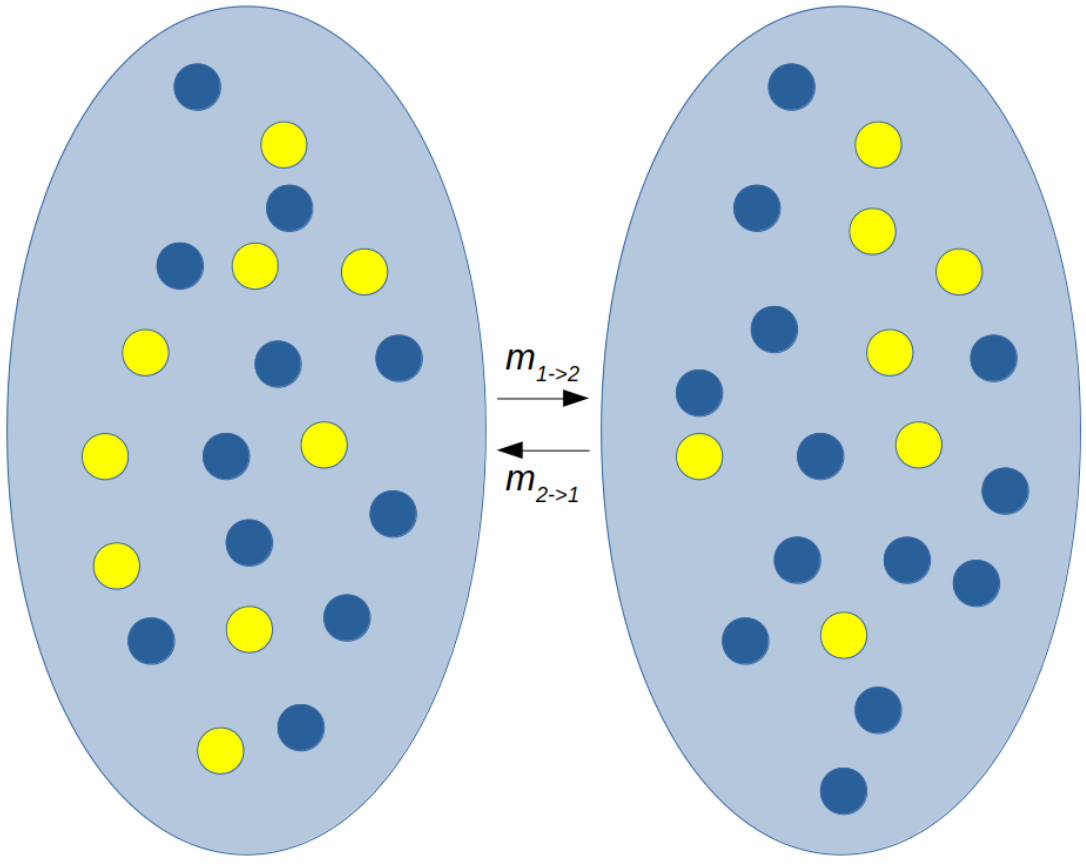
\includegraphics[width=.45\textwidth]{graphics_day2b_popgen/rates_gene_flow.png}
	\end{center}
	\caption{An individual from one population is replaced with an individual from the other with probability $m$ (migration rate).}
	\end{figure}
\end{frame}
%%%%%%%%%%%%%%%%%%%%%%%%%%%%%%%%%%%%%%%%%%%%%%%%%%%%%%%%%%%%%%%%%%%%%%%%%%%%%%%%%%%%%%
%
%
%
%%%%%%%%%%%%%%%%%%%%%%%%%%%%%%%%%%%%%%%%%%%%%%%%%%%%%%%%%%%%%%%%%%%%%%%%%%%%%%%%%%%%%%%
\begin{frame}\frametitle{$F_{ST}$ and migration rates}
	Using the coalescence theory assuming an infinite sites model, we can derive that
	\begin{equation}
		F_{ST} = \frac{1}{1 + 4Nm_T}
	\end{equation}
	with $m_T$ being the total number of migrants.
	\begin{center}
		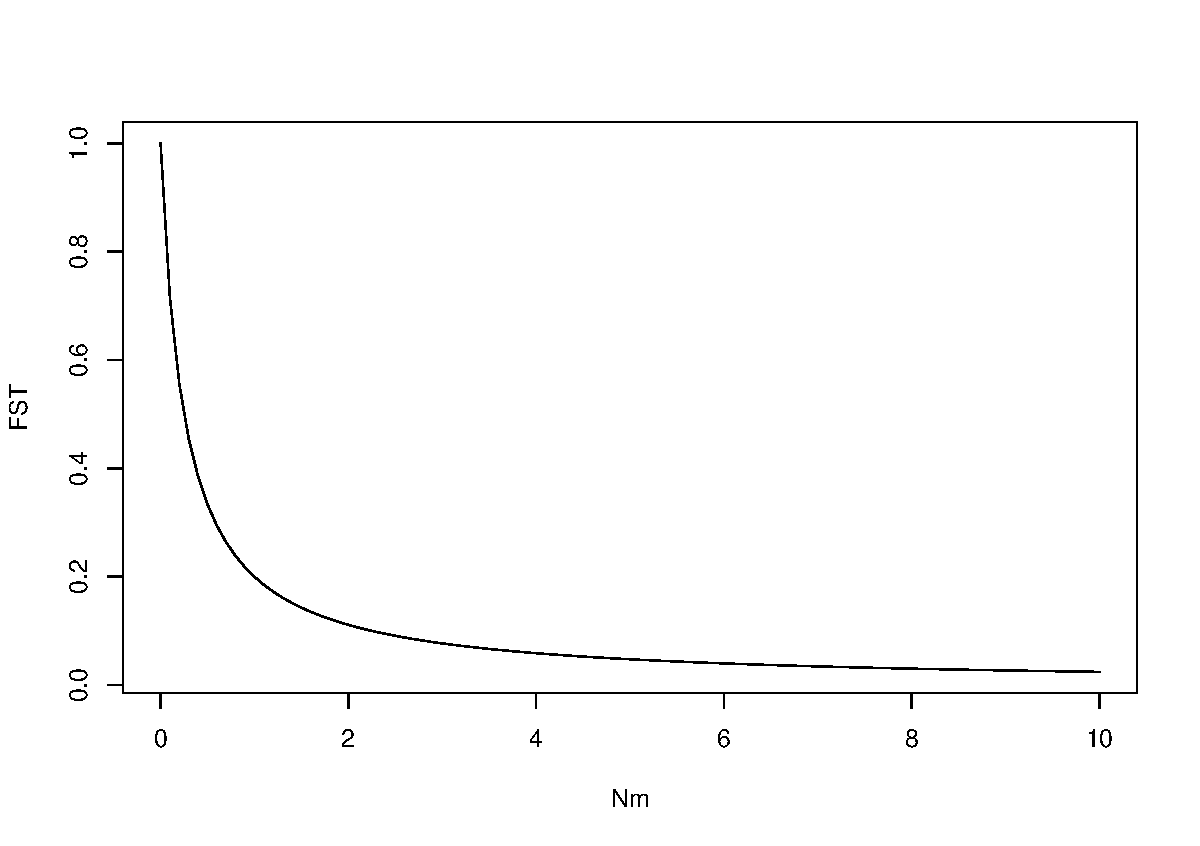
\includegraphics[width=.55\textwidth]{graphics_day2b_popgen/F_ST.pdf}
	\end{center}
\end{frame}
%%%%%%%%%%%%%%%%%%%%%%%%%%%%%%%%%%%%%%%%%%%%%%%%%%%%%%%%%%%%%%%%%%%%%%%%%%%%%%%%%%%%%%
%
%
%
%%%%%%%%%%%%%%%%%%%%%%%%%%%%%%%%%%%%%%%%%%%%%%%%%%%%%%%%%%%%%%%%%%%%%%%%%%%%%%%%%%%%%%%
\begin{frame}\frametitle{``Island'' model}
	\begin{block}{}
		It assumes that populations have been subdivided for a very long time so that an equilibrium has been established and that then there is ongoing \textbf{gene-flow}.
	\end{block}
	It is not a realistic model for some species.
	\begin{center}
		\includegraphics[width=.65\textwidth]{graphics_day2b_popgen/island_model_map.png}
	\end{center}
\end{frame}
%%%%%%%%%%%%%%%%%%%%%%%%%%%%%%%%%%%%%%%%%%%%%%%%%%%%%%%%%%%%%%%%%%%%%%%%%%%%%%%%%%%%%%
%
%
%
%%%%%%%%%%%%%%%%%%%%%%%%%%%%%%%%%%%%%%%%%%%%%%%%%%%%%%%%%%%%%%%%%%%%%%%%%%%%%%%%%%%%%%%
\begin{frame}\frametitle{Divergence model}
	\begin{block}{}
		It describes populations diverging from common ancestral populations without subsequent gene-flow.
	\end{block}
	\begin{figure}
	\begin{center}
		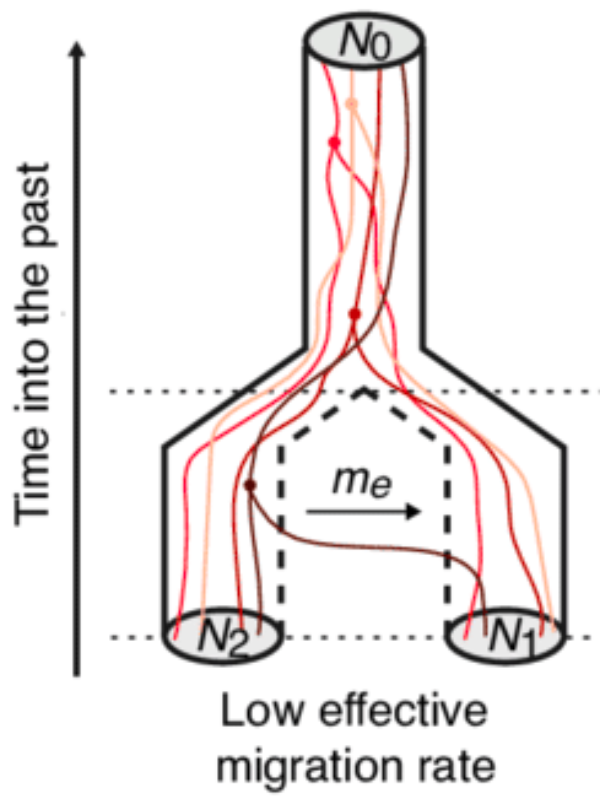
\includegraphics[width=.25\textwidth]{graphics_day2b_popgen/divergence_model.png}
	\end{center}
	\caption{TMRCA overestimates the divergence time.}
	\end{figure}
\end{frame}
%%%%%%%%%%%%%%%%%%%%%%%%%%%%%%%%%%%%%%%%%%%%%%%%%%%%%%%%%%%%%%%%%%%%%%%%%%%%%%%%%%%%%%
%
%
%
%%%%%%%%%%%%%%%%%%%%%%%%%%%%%%%%%%%%%%%%%%%%%%%%%%%%%%%%%%%%%%%%%%%%%%%%%%%%%%%%%%%%%%%
\begin{frame}\frametitle{Isolation by distance}
	\begin{block}{}
		The degree of population subdivision increases with geographical distance.
	\end{block}
	\begin{itemize}
		\item Migration rate is a linear function of geographical distance.
		\item Migration occurs only between adjacent populations (stepping-stone models).
		\item Series of divergence events (sequential colonisation).
	\end{itemize}
\end{frame}
%%%%%%%%%%%%%%%%%%%%%%%%%%%%%%%%%%%%%%%%%%%%%%%%%%%%%%%%%%%%%%%%%%%%%%%%%%%%%%%%%%%%%%
%
%
%
%%%%%%%%%%%%%%%%%%%%%%%%%%%%%%%%%%%%%%%%%%%%%%%%%%%%%%%%%%%%%%%%%%%%%%%%%%%%%%%%%%%%%%%
\begin{frame}\frametitle{Isolation by distance}
	\begin{figure}
	\begin{center}
		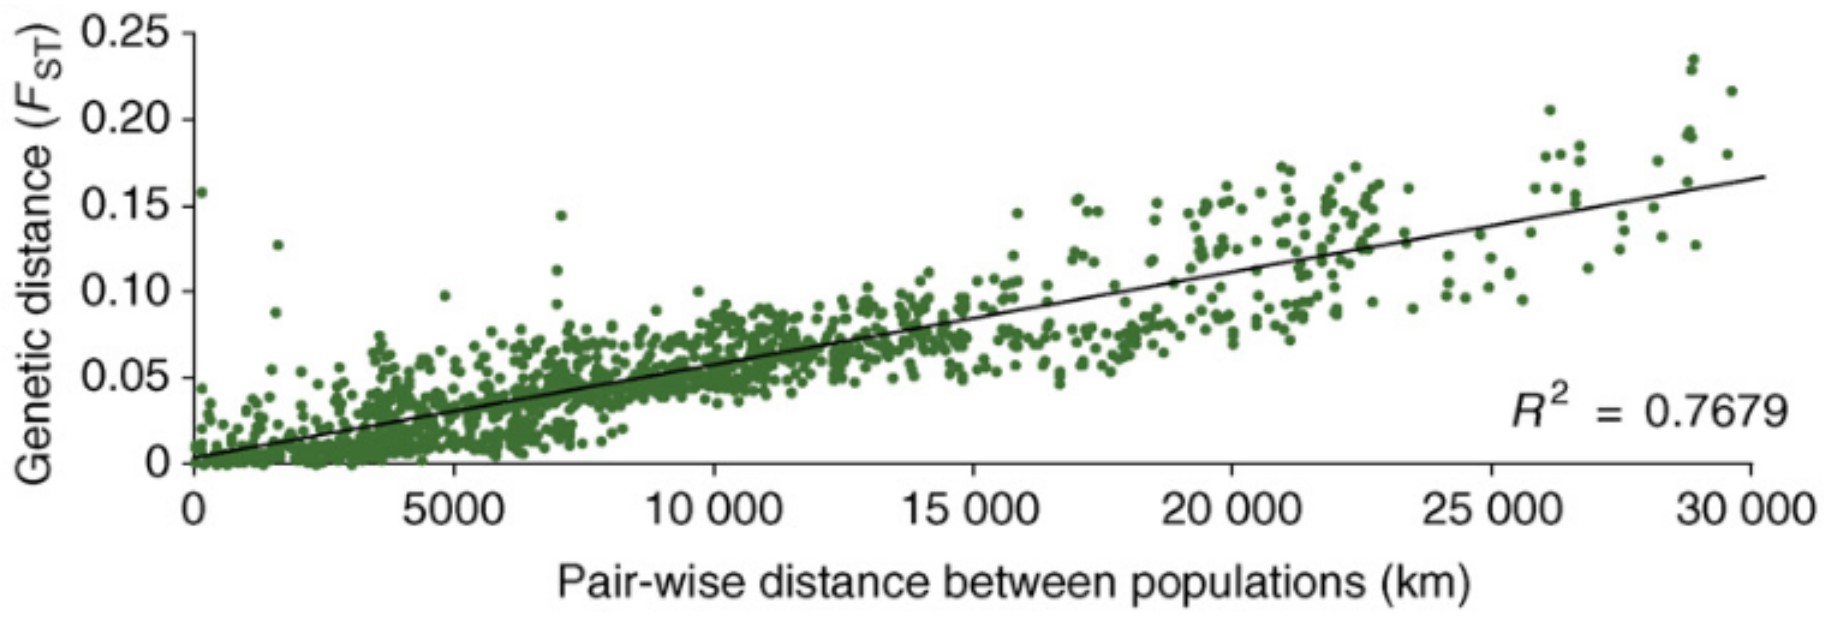
\includegraphics[width=.8\textwidth]{graphics_day2b_popgen/isolation_by_distance.png}
	\end{center}
	\caption{Isolation by distance in human populations.}
	\end{figure}
\end{frame}
%%%%%%%%%%%%%%%%%%%%%%%%%%%%%%%%%%%%%%%%%%%%%%%%%%%%%%%%%%%%%%%%%%%%%%%%%%%%%%%%%%%%%%
%
%
%
%%%%%%%%%%%%%%%%%%%%%%%%%%%%%%%%%%%%%%%%%%%%%%%%%%%%%%%%%%%%%%%%%%%%%%%%%%%%%%%%%%%%%%
\begin{frame}\frametitle{Intended Learning Outcomes}
	\textbf{Population subdivision}\\[2ex]
	In this lecture you have learned to
	\begin{itemize}
		\item Quantify the effect of population subdivision on allele frequencies and heterozygosity.
		\item Calculate measures of population genetic differentiation.
		\item Discuss divergence models.
	\end{itemize}
\end{frame}
%%%%%%%%%%%%%%%%%%%%%%%%%%%%%%%%%%%%%%%%%%%%%%%%%%%%%%%%%%%%%%%%%%%%%%%%%%%%%%%%%%%%%%
%
%
%
%%%%%%%%%%%%%%%%%%%%%%%%%%%%%%%%%%%%%%%%%%%%%%%%%%%%%%%%%%%%%%%%%%%%%%%%%%%%%%%%%%%%%%
\end{document}
